\documentclass{report} 
\usepackage[utf8]{inputenc}
\usepackage{graphicx}
\usepackage[margin=1.5in]{geometry}
\usepackage{lingmacros}
\usepackage{verbatim}
\usepackage{subfig}
\usepackage{wrapfig}
\usepackage{tipa}
% exempel: 2) Inte vet jag
%              not know I
%             I don't know

\begin{document}
% ska gå att förstå och locka till läsning
%ska tydligt beskriva vad rapporten handlar om
%ska innehålla vettiga sökord
\title{Scaling up a GF grammar for free parsing} %A nice titleScaling up a GF grammar and preparing it for cool stuff for Swedish}
\author{Malin Ahlberg}
\maketitle
\newpage


\abstract{
This is the report of the work of expanding and enhancing a GF grammar and preparing
it for parsing of free Swedish. 
Outside of this project, an equivalent project for English is being worked upon,
as are tehcniques for making the parser robust.
With this in mind, we have extended the current GF grammar to adapt it for
Swedish specifically so that it can parse an extended set of basic
constructions. We have completed a method for importing the electronical 
lexicon Saldo to a GF format and established a connection to the treebank Talbanken.
The imported lexicon consists of more than 100 000 words
and the grammar now covers ??\% of the xx part of Talbanken. 
% The mapping between the annotations of Talbanken and GF is automatic. 
% The goal is to build a robust parser dealing with uncontrolled natural
%language, a parser which can parse all of Talbanken.

% sf dream to be able to work with npl. Parser important, statistics working
% on n-grams fail, closer to the human brain with rules? 
% Describe the basic.. of Swedish, in a format compatible with 20 other languages.
% example of sentence and how it can be parsed, stepping out of the controlled lang.
% Combine other resources, create free software.
% Equivalent for English and other languages coming.
% We aim for free parsing, this is preparation and up-scaling, finding difficulties.
}

\newpage

\section*{Acknowledgments}
% Ramona, Aarne, Elisabet, Markus, Peter?, Lars, Dan, Krasimir etc
% Funding!

% check references! lncs is good maybe. lnai
\newpage

\tableofcontents
\newpage
\chapter{Introduction}
%>> short intro to GF
The grammar formalism GF has so far been succesfull used for 
controlled languges, but recent experiments have showed
that it is also possible to use the framework for parsing free language.
Parsing, that is the task of automatically identifiyng morpohlogical and
syntactical structures to text, is subject to increasing interest, especially
considering the steadily growing amount of data available online. 
So far there is no freely available grammar-driven parser that give a deep analyse for
Swedish. The fact that the existing rule-based Swedish
parsers are not freely available does not only restrict their
usage but also their possiblities of being developed. Our
goal is
to create a open source Swedish grammar and parser that can be continuosly enhanced and
be made use of in other projects.\\
To build a parser or a grammar from scratch is a heavy work ~~ and we
therefore combine already existing resources.
We start from GF resource grammar and thereby get
%The usage of GF allows us to start from
a well-defined system for describing grammar, as well as a strong connection to
more than 20 other langugages implentented in the framework.
%>>The grammar defines a parser, which accepts all constructions defined by the grammar.


\section{Aims}
%>> enhance gf...
The purpose of this project has been to prepare the GF grammar for free parsing.
This has meant to develop earlier techniques to fit for Swedish, create methods
for achieving and keeping a extensive lexicon and to adapt the existing
resource grammar to fit for more language specific constrictions.
We hence needed to extend the Swedish grammar to cover
the language specific constructions. Further a large lexicon was
needed, as well as a method for evaluation.
During this project, we have worked on and explored those things and
while identifying problems and future work.


\section{Outline}
This thesis is divided into 6 chapters. We start by giving some background
information to areas relevant to the project. %Chapter \ref{sec:background} 
Grammatical Framework is presented in section \ref{sec:gf} and a deeper
presentation of the Swedish resource grammar is given in section \ref{sec:swegf}.
Section \ref{sec:swedish} gives an introduction Swedish and
brief presentations of Saldo and Talbanken are found in section \ref{sec:saldo} and
\ref{sec:talbanken} respectively.
A summary of related work can be found in section \ref{sec:related}.

Chapters \ref{sec:prog.saldo} - \ref{sec:Mapping} present the methodology,
implementation and some results. Finally, conclusions, an evaluation and a list
of future work are presented in chapter \ref{sec:results}.

%We have extended the Swedish resource grammar in GF, to give a better coverage and imported
%a large lexicon. Work to compare the trees from Talbanken to GF and to translate them.


%Ultimate goal: want computers to 'understand' language. Not good with flat strings.
%We need to translate strings of natural language to a richer structure,
%a parse tree. 
%There are parsers which put only put part-of-speach tags to
%the text, and others that gives a deeper analyse. 
%There are statistical parser, and parser which only are deal with controlled language.
%The GF parser are one of those. 
%What is parsing, flat strings to trees, example picture, what is deep parsing.

%What is controlled language,
%what is robust parsing and why we need it for free langugae, benefits of a grammar.
%GF is grammar formalism, many languages, many projects for controlled lang.
%GF grammar for Swedish, how big, not intended for parsing, but for building
%application grammars. Experiments of using the grammar for free parsing, methods
%being developped for this. Benefits of starting from GF. Free parsing is
%interesting. To do this, we need a better (bigger grammar), a large scale
%lexicon, and an evaluation method. This project has explored those things. The
%grammar also have other usages, important in itself, so we wanted to make it as
%covering as possible without being overallowing or too ambiguous.

%What we could not cover by this project, what have been covered before (in
%the spring project), and why we choose those parts.

\chapter{Background}  
\label{sec:background}
The work described in this is thesis is part of a bigger project which aims at
using GF for parsing free Swedish. 
In previous work \ref{??} the start on extending the Swedish GF grammar was
made and a tool for lexical aquistion were developed.
We now construct a bigger
and more expressive grammar as well as a large scale GF lexicon.
As all GF grammars, this one can be used for parsing, and we develop it by getting
examples, ideas and test material from a treebank.
The project is hence heavily depending on three resources, which will be described
in this section.


\section{Swedish}
\label{sec:swedish}
>> move, have GF first?\\
Swedish \cite[Inl. \textsection 3]{SAG}is a North-Germanic language,
closely related to Norwegian and Danish. The languages share most of their
grammatical structures and are mutually intelligible. Swedish is also 
an official language in Finland and altogether spoken by approximately 10 ~~
9?Check SAG million people.
Swedish syntax is often similar to English, but have some characteristics ~~:

\subsection*{Post-nominal articles} 
Unlike most of the world's languages Swedish express not only the number but also
the definitness of a noun by suffixes. The endings are decided by the gender of the noun,
which may be \textit{neuter} or \textit{common}.\\
%(or \textit{utrum}) 

\begin{tabular}{l|lll}
&\textbf{Definite}& \textbf{Indefinite}& \textbf{Gender} \\
 \hline
\textbf{Singular} & {en katt} & {katten} & \textit{common}\\
& \emph{a cat} & \emph{the cat} &\\
\textbf{Plural} & katter & katterna &\\
 &\emph{cats} & \emph{the cats} &\\
 \hline
\textbf{Singular} & {ett hus} & {huset} & \textit{neuter}\\
 & \emph{a house} & \emph{the house} & \\
\textbf{Plural} & hus & husen & \\
& \emph{houses} & \emph{the houses} & \\
\end{tabular}\\

The definiteness can be accentuated by using the definite articles.\\

\begin{tabular}{llll}
den katten & det huset & de katterna & de husen \\
\emph{the cat} & \emph{the house} & \emph{the cats} & \emph{the houses} \\
\end{tabular}\\

The definite articles are required when the noun is modified by adjectival phrase, sentence
\ref{sent:trottkatt}b is hence not grammatically correct.
%\enumsentence{\shortexnt{4}
%{Den& trötta& katten & sov}
%{the& tired& cat+\textbf{the} & slept}}
\enumsentence{\begin{tabular}{llllll}
a.& Katten sov. & b.& *Trötta katten sov &c. &Den trötta katten sov\\
&The cat slept. & &~~The tired cat slept& &The tired cat slept\\
\end{tabular}}\label{sent:trottkatt}

%can be superdoubled
%example: den där boken


\subsection*{Verb second}
Swedish is a verb-second language \cite[p.116]{gunlog}: the
second constituent of a declarative main clause must consist of a verb.
The normal word order is subject-verb-object, but any syntactic category can be
fronted \cite[\textsection 1027]{H&H}.
Topicalisation is very common, especially for temporal and spatial adverbial phrases.
The examples \ref{ex:swedish-svo} - \ref{ex:swedish-avso} all have the same propositional
meaning, but vary in how the content is presented.
%~~ although the fronted part of sentence \ref{ex:swedish-ovs} and \ref{ex:swedish-avso} are being
%emphasized.
\enumsentence{
\shortex{4}
{Du & ser &  inte &mig.}
%empha glossning!! ha samma överallt, ' eller ''
{you & see & not & me}
{`You  don't see me'.}} \label{ex:swedish-svo}
\vspace{-3mm}
\enumsentence{
\shortexnt{4}
{Mig  & ser &  du & inte.}
{me & see & you & not}}\label{ex:swedish-ovs} 
\vspace{-3mm}
\enumsentence{
\shortexnt{4}
{Inte & ser& du &mig.}
{not&  see& you& me}} \label{ex:swedish-avso}

%Alla syntaktiska kategorier kan be fronted utom obetonade satsadverbial (ju,väl).
%\enumsentence{
%\begin{tabular}{lll}
%  Johan & gick & sakta på gatan.\\
%\emph{Johan} & \emph{walked} & \emph{slowely on the street.}\\
%  Sakta & gick & Johan på gatan.\\
%\emph{Slowly} & \emph{walked} & \emph{Johan on the street.}\\
%  På gatan & gick & Johan sakta.\\
%\emph{On the street} & \emph{walked}  & \emph{Johan slowly.}\\
%\end{tabular}}

Inverted word order marks questions
\enumsentence{
\shortex{4}
{Såg & du & mig & inte?}
{saw  & you&  me& not}
{`Didn't you see me?'}}
%\enumsentence{Gick Johan på gatan?\\
%        \emph{Did Johan walk on the street?}}
The word order in subordinate clauses in also slightly different,
%>> and stricter
\enumsentence{Main sentences:\\
{\shortex{8}{Jag & såg & Anna & men & hon & såg & {\bf inte} & mig }
{ I & saw & Anna & but & she & saw & {\bf not} & me}
{`I saw Anna but she didn't see me'}}}
\enumsentence{Subordinate sentence:\\
\shortex{7}{Jag & förstod & att& Anna& \textbf{inte}& såg& mig.}
            {I &  understood & that& Anna& \textbf{not}& saw& me}
            {`I understood that Anna didn't see me'}} 

\subsection*{Passive voice}
There are two ways of forming passive verb phrases in Swedish: the 
\textbf{periphrastic passive}, formed by using a modale auxiliary verb \\
%>> better with animate subjects
\enumsentence{
\shortex{5}
{Tjuven &blev& tagen& av & polisen}
{the thief & was & taken & by & the police }
{`The thief was arrested by the police'}}
\label{gfPass:peri-pass}
and the \textbf{s-passive} which is formed by adding an \emph{s} to the verb: \\
\enumsentence{Passive \hspace{45mm} Active\\
\shortexm{12}
{Tjuven & togs&  av & polisen}
{the thief&  took+\textbf{s}&  by&the police}
{`The thief was arrested by the police'}
{&&Polisen & tog & tjuven}
{&&the police & took & the thief}
{\hspace{-9mm}`The police arrested the thief'}}
\label{gfPass:s-pass}
The s-passive is the most commonly used one for both written
and Swedish \cite[??]{SAG} and dominates especially when the subject is inanimate.
%cf.
%\enumsentence{
%\shortex{5}{Ett & lejon & jagade & honom.}
%        {A &lion &hunted &him.}
%        {`A lion was hunting him.'}}

\subsection*{Impersonal constructions}
Constructions with `det är/var' (\emph{`it is/was'}) is very common in Swedish \cite[\textsection 309d]{H&H}:
\enumsentence{
\shortex{6}{Det & var & roligt & att & höra.}
{it &was & nice &to &hear.}
{`I'm glad to hear that.'}}
'Det' (\emph{it}) is also used as formal subject in presentational constructions where
the real subject is put in the position of an object.
\enumsentence{
\shortex{6}{Det &står &en &älg &på &fältet.}
{ it & stands &a & moose &on &the field}
{`There is a moose in the field.'}}

\subsection*{Reflexive pronouns}
\label{swe:refl}
The Scandinavian language have special reflexive pronouns
and possessive pronouns for the 3rd
person \cite[\textsection 310 \& 319]{H&H}. They are distinct from the normal 3rd person forms.
\enumsentence{
\begin{tabular}{llll}
a. & Han slog \textbf{sig}.&\hspace{20mm}b. & Han såg \textbf{sitt} barn.\\
&\emph{He hit him self.} && \emph{He saw his (own) child.}
\end{tabular}}
\enumsentence{
\begin{tabular}{llll}
a. &Han slog \textbf{honom}. &b.& Han såg \textbf{hans} barn.\\
&\emph{He hit him (another person).}&&\emph{He saw his (another person's) child.}
\end{tabular}}
The 1st and 2nd persons use the normal personal pronoun in object form as reflexive
pronouns.

%Mention varandra. Same idea.
%Basic info about Swedish. V2 lang, inverted word order and subordinate clauses.
%Passive, reflexive 'sitt', 'det är', 'det sitter en katt där', prepare the reader
%for what will be written in the grammar part.
%Adjectives but not verbs congruate with nouns. De är stora, They are big, Jag
%är stor, I am big
%Since the s-passive is the most common one in written Swedish \cite{SAG-34-1}, it has


\section{Saldo}
\label{sec:saldo}
A good parser needs a good lexicon. We have used of Saldo \cite{saldo}, a
large electronic lexicon developed and maintained at Gothenburg University. It is
built on Svenskt Associations Lexicon and contains information about more than 
120 000 modern Swedish words.
The ~~words are equipped ~~ with semantic, syntactic and a morphological
information. The user can find compounding analyses, examples of usage in corpora,
and graphs of semantically connected words.\\
\begin{figure}[h!]
\centering
\subfloat[Morphological info for ``katt"]{\label{pic:saldoTab}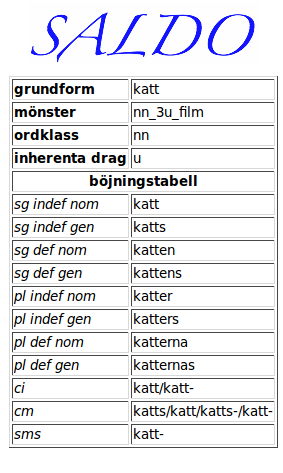
\includegraphics[width=40mm]{saldotab.png}}
\hspace{20mm}
\subfloat[Graph showing the hyponyms of ``katt"]{\label{pic:saldoWheel}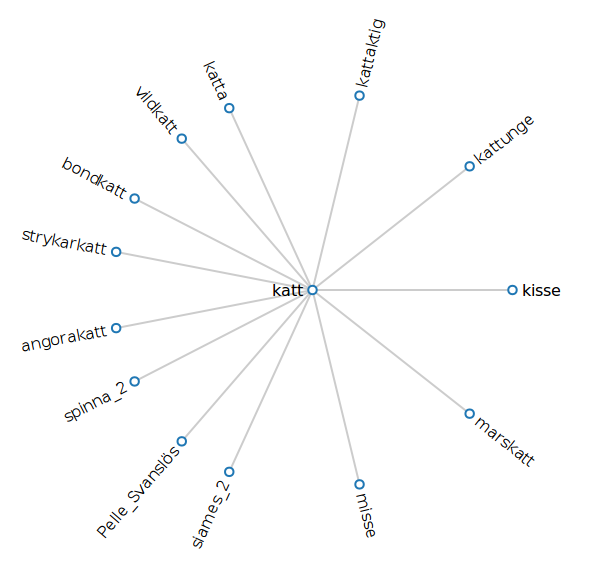
\includegraphics[width=70mm]{saldograph.png}}
\caption{Information in Saldo}
\label{fig:saldo}
\end{figure}

If one word has different meanings, there will be separate entries for each of
them.  The word ``växa" (``grow") for example, has two meanings: \emph{getting
bigger}
\enumsentence{Gräset växte varje dag\\
The grass grew each day}
or \emph{being a plant}. 
\enumsentence{Det växte en gammal ek där.\\
There stood an old oak.}
The word ``växa" is however declined the same way for both interpretations of the word.
Hence Saldo's morphological lexicon, provided under LPGL in XML format,
only keeps one entry of ``växa".
For the homonyms that do not share the whole inflection tables, different entries are 
kept in the morphological lexicon.

For our purpose, only the morphological lexicon was needed.
The data can be processed and translated to GF format as described in 
section \ref{sec:prog.saldo}.

\section{Grammatical Framework}
\label{sec:gf}
The main component of the the project is the Grammatical Framework (GF) \cite{gfbok}, %It is
a grammar formalism based on Martin-Löf type theory \cite{martinlof}. GF is
designed for multilingual applications and the formalism is 
%equivalent to Parallel Multiple Context-Free Grammars (Seki \& al. 1991), an instance of
%generalized context free grammar (GCFG) it is hence
stronger than mildly contex-free grammars and hence has the same expressiveness
as Tree Adjoining Grammars (Joshi,1975) and Head Grammars (Pollard,1984).

GF is a strongly typed functional programming languages, inspired by
%programming languages like 
ML \cite{ml} and Haskell \cite{haskell}. The logic and reasoning 
are inspired by \textlambda Prolog \cite{prolog} and 
by Agda \cite{agda}, with which GF also shares its type checking algorithm.
The first version of the framework was implemented by the Xerox Research Center
in Grenoble and is now mainly developed in Gothenburg. On of the biggest
achivements is a library covering the 
basic morphological and syntactical structures of more than
20 languages (see section \ref{sec:resources}).


%> dependent and implicit types : agda. (read gf book and krasses book)
A grammar written in GF can be used for both parsing and generation.
The parsing algorithm is incremental and has polynomial time and space
complexity \cite{gfMech}. 
The GF package also provides various tools for working with and using the grammars:
a compiler, an interpreter and a runtime system.
The grammars can be compiled into portable grammar format (PGF) \cite{pgf},
which can be used with %There are libraries for using PGF files with
Java, Java script, C and Haskell. 
%>> Haskell only complete, also or C\# and C.  %may also be used in Android applications.
The interpreter, the GF shell, allows
the user to try and test her grammar by using commands for parsing, vizualization of parse trees,
random generation, word alignment, morphological quizzes etc.
%The following example shows how to parse a sentence and visualizing the parse tree.
%, by using the \textit{pipe} \verb-|-, sending the result to 
\begin{figure}[h]
\begin{verbatim} 
> parse "jag ser katten" | visualize_parse -format=pdf -view=evince
> parse "jag ser katten" | visualize_tree  -format=pdf -view=evince
\end{verbatim}
\caption{Example of how the GF shell can be used. The first command will parse the given
sentence and visualize the resulting parse tree and the second will visualize the 
abstract syntax tree.}
\label{fig:shellvp}
\end{figure}
\begin{figure}[h]
\centering
\subfloat[GF abstract tree]{\label{pic:gfAtree}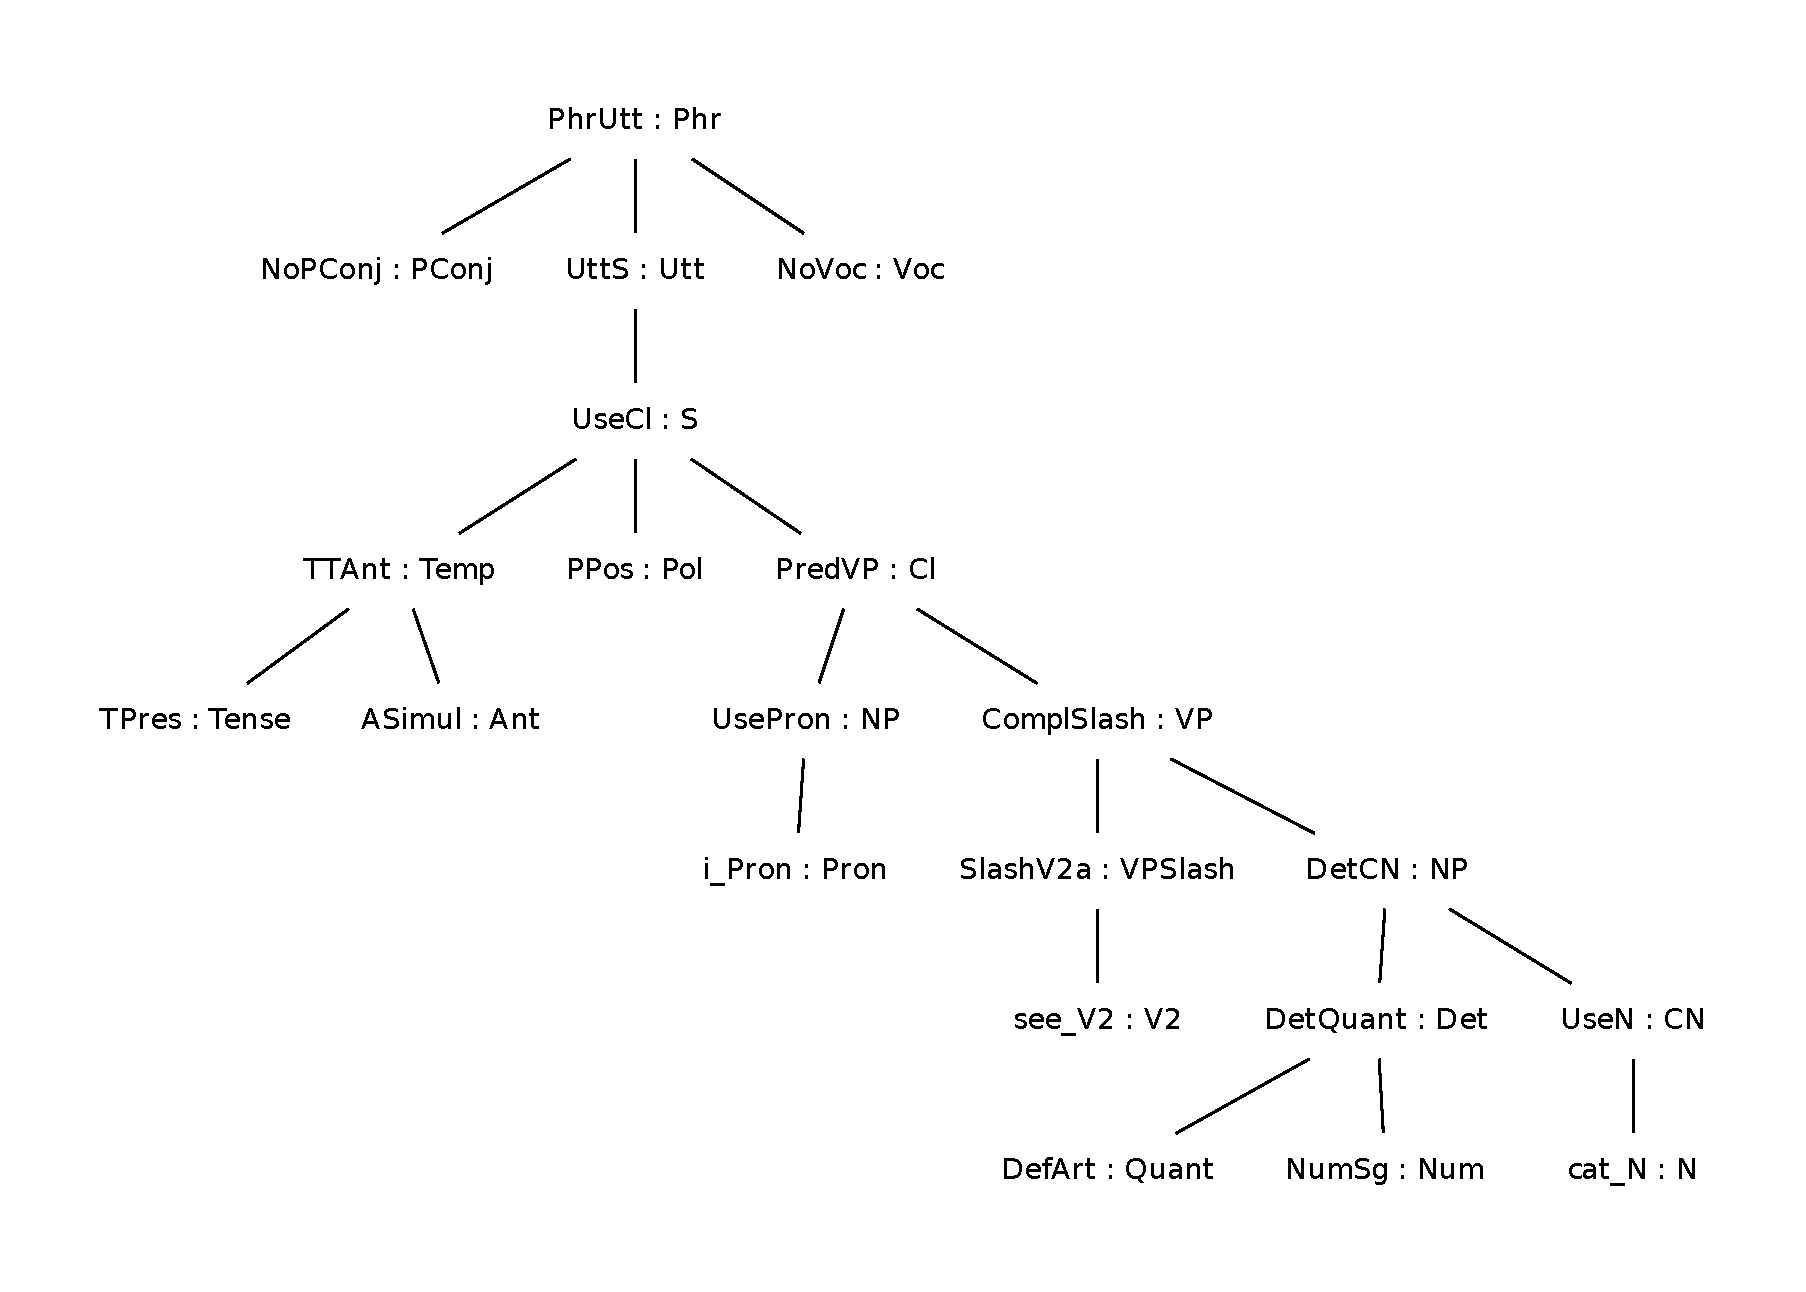
\includegraphics[width=100mm]{gfTree.pdf}}
\subfloat[Swedish parse tree]{\label{pic:gfStree}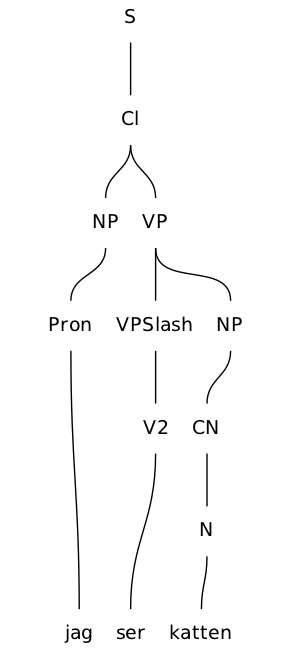
\includegraphics[width=30mm]{gfSTree.png}}
\caption{Parse tree and abstract tree for the sentence ``Jag ser katten".}
\label{fig:gftree1}
\end{figure}

% nice: test vt -format=pdf -view=evince -nofun
\begin{wrapfigure}{l}{0.3\textwidth}
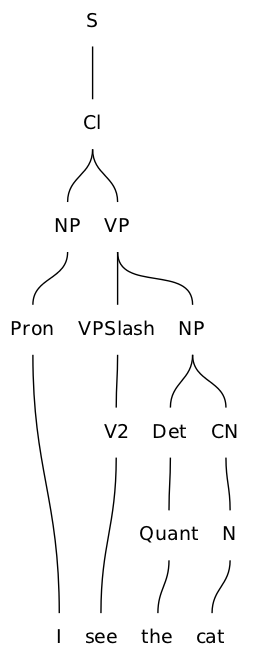
\includegraphics[width=20mm]{gfETree.png}
\caption{English parse tree}
\label{pic:gfEtree}
\end{wrapfigure}

The visualization of the trees is done with graphviz\footnote{http://www.graphviz.org/}.
Figure \ref{fig:gftree1} shows the results from running the commands in figure \ref{fig:shellvp}
A GF parse tree has two visualized representations, the \textit{parse tree} and
the \textit{abstract tree}.
The abstract trees shows all functions GF needs to use
to parse the sentence.
% do not know about abstract/concrete yet: and is consequently the same for all concrete syntaxes.
The parse tree (\ref{pic:gfStree}) shows the words and which types
the functions assign to them.
The reader should keep in mind that the visualized parse trees is not a
complete representation.
If the end node of a  branch has no corresponding word, it is excluded from
the visualized parse tree. This is the case for the definite article in Swedish,
and the information \verb-DetQuant DefArt NumSg- is not shown in figure \ref{pic:gfStree}.

In the corresponding English parse tree, figure \ref{pic:gfEtree},
the article \emph{``the"} is explicit and therefore shown as a quantifier in the parse tree.\\

%>> how parse trees work, not correct complete representation.
%>> not a constituent structure. compare to lfg, fstructure, cstructure.

%>>the scope is controlled language, but possible ambiguities (discuss this in future
%>>work, saldo, conclusion). Ambiguities: from multilinguality, or inherited:
%>>syntactical (man with the telescope), lexical (youSg/Pl, växa).
%>> have ambiguity section. 
The scope of GF grammars is usually controlled language. By
restricting the coverage, the number of ambiguities
can be limited and we can ensure that the semantics is preserved during
translation. The inhereted ambiguities and the ones arising from multilinguality will
of course remain, but can be controlled more easily. %Example of domainspecific word?
The use of controlled language gives a possibility of good and reliable translation.
  Some examples of projects using GF are WebAlt \cite{webalt},
a project which aims to develop language independent material for mathematics problems,
and the formal software verification tool KeY \cite{key}, in wich GF is used for
translating specification to natural language.
%>> key, talk, hats, bom (see references in Ramonas thesis).
%>> use talk here and move key to other place??
The framework is also used in the
European project MOLTO \cite{molto} for online translation between up to 15 language.\\


\subsection{Writing a GF grammar}
The key feature in GF is the distinction between
\textit{abstract} and \textit{concrete} syntax. The abstract syntax represents
the internal structure and models the semantics without concern for language
specific features such as agreement or word order.
One abstract grammar can be implemented by a number of concrete grammars, each
representing one language. As a comparison, the abstract and concrete syntax
may be thought of as fstructures and cstructures in Lexical Functional Grammar (Bresnan and Kaplan, 1982).

%Being developed with multilinguality in mind, GF makes an important 
\begin{figure}[h]
\begin{verbatim}
 abstract TestGrammar = {
  cat N ; V ; S ;

  fun 
    Pred : N -> V -> S ;
    cat_N : N ;
    sleep_V : V ;
 }
\end{verbatim}
\caption{A small example of an abstract syntax}
\label{fig:gfAbstract1}
\end{figure}

The example in figure \ref{fig:gfAbstract1} shows an abstract grammar defining three categories, % \verb|Categories|,
one for nouns, one for verbs and one for sentences. An abstract grammar also gives
the types of functions. In our case we have \verb|Pred| which
tells us that by taking a noun and a verb we can form a sentence. At this stage, 
no information of how this is done is given. The grammars also defines two words,
the noun \verb|cat| and the verb \verb|sleep|. 

% or how any of the categories should look.
\begin{figure}[h]
\begin{verbatim}
concrete TestGrammarSwe of TestGrammar = {
  lincat N, V, S = Str ;
   
  lin Pred n v   = n ++ v ;
      cat_N   = "katten"  ;
      sleep_V = "sover"  ;
}
\end{verbatim}
\caption{A Swedish concrete grammar}
\label{fig:gfSweCnc1}
\end{figure}

%>> move much of this to Swedish GF part?
Figure \ref{fig:gfSweCnc1} shows how the abstract grammar can be implemented
for Swedish. Nouns, verbs and sentences are all defined as strings, \verb|Str|,
and \verb|Pred| simply glues the two strings ``katten" and ``sover" together:\\
\verb|Pred cat sleep = "katten sover"|.\\
We get a more complicated example if we allow the nouns to be used in both
plural and singular. We add a category \verb|NP| to the
abstract. Note that \verb-NP- is normally used for nouns with a fixed definitness, but for 
now we concentrate on the number only. Hence \verb|N| now means a noun
in any of the number, and we introduce two function, \verb|NSg : N -> NP| and
\verb|NPl : N -> NP| which sets the number.
\begin{figure}[h!]
\begin{verbatim}              
 abstract TestGrammar = {          concrete TestGrammarSwe of TestGrammar = {
  cat N ; NP ; V ; S ;               lincat V, S, NP = Str ;
                                            N = {s : Num => Str} ;
  fun                                lin   
    Pred : NP -> V -> S ;              Pred n v = n ++ v ;
    NSg : N -> NP ;                    NPl n = n.s ! Pl ;
    NPl : N -> NP ;                    NSg n = n.s ! Sg ;
    cat_N : N ;                        cat_N = {s = table {Sg => "katten" ;
    sleep_V : V ;                                          Pl => "katterna"}};
 }                                     sleep_V = "sover"  ;
                                     param Num = Sg | Pl ;
                                     }
\end{verbatim}           
\caption{A modified grammar}
\label{fig:gfTest2}
\end{figure}
Figure \ref{fig:gfTest2} introduces some new concepts: records,tables and parameters.
In the concrete syntax, \verb|N| is defined to be a record consisting of the field
\verb|s|. The type of \verb|s| shows that it is a table, which given a
parameter of type \verb|Num| returns a string. \verb|Num| is defined as a
parameter, which can either have value \verb|Sg|
or \verb|Pl|. In \verb|NPl| and \verb|NSg|, \verb|n.s| means that we use the
field \verb|s| of \verb|n|, and then the selection operator \verb|!| is used to
select a branch in the table.

If we want to implement a English version of the grammar, we encounter another
problem: the verb form depends on the noun phrase. The \verb|NP| needs to carry
information about which number it is in, and \verb|Pred| can pass this on to the
verb. Hence, the \verb|V| also needs to be a table, depending on the number.
\begin{figure}[h!]
\begin{verbatim}              
concrete TestGrammarEng of TestGrammar = {
  lincat S = Str ;
         V = {s : Num => Str} ;
         N = {s : Num => Str} ;
         NP = {s : Str ; num : Num} ;
  lin   
    Pred n v = n.s ++ v.s ! n.num ;
    NPl n = {s = n.s ! Pl ; num = Pl} ;
    NSg n = {s = n.s ! Sg ; num = Sg} ;
    cat_N = {s = table {Sg => "the cat" ;
                        Pl => "the cats"}};
    sleep_V = {s = table {Sg => "sleeps" ; 
                          Pl => "sleep"}};
  param Num = Sg | Pl ;
  }
\end{verbatim}           
\caption{English implementation}
\label{fig:gfTestEng}
\end{figure}

%maybe continue example with swedish and english, have DetNP : N -> N wich
%gives 'the cat', 'katten'. Thereby introduce tables, parameters, fields.
%Show abstract tree.

We now have two implementations of the abstract. The resulting GF grammar is able to
both parse a string to a abstract tree and to go in the other direction; to produce
a string of natural language given an abstract tree. This step is called linearization.
Translation is a consequence of this, we can parse a Swedish string and then 
linearize the resulting abstract tree to English. 

Valency information is normally built into the GF categories. To indicate that
a verb is transitive and needs an object, we use the category \verb_V2_.
\begin{verbatim}
abstract:
cat V2 ; 
eat_V2 : V2 ;
rat_N ;
UseV2 : V2 -> NP -> V ;

concrete:
eat_V2 = "äta" ;
rat_N = {s = table {Sg => "råttan" ;
                    Pl => "råttorna"}};
UseV2 v np = v ++ np ;
\end{verbatim}

The example above now allows ``Katten äter råttan", but not ``Katten äter".
\verb|UseV2| concatenate the strings ``äter" and ``råttan". Note that if we
wanted to add negation, ``katten äter inte råttan", or question "äter katten råttan",
we cannot glue the verb to the object at once. Instead we would have to use a table,
with one field for the verb and one for the object. 

\subsection{The resource library}
\label{sec:resources}
%>>Best part? Biggest library?
%>>Most general resource, first large grammar, covers fundamental syntactics.
The GF package provides a powerful resource library \cite{gf-resource}, which covers the
fundamental morphology and syntactics for more than 20 languages. %is a very useful part of the framework. It is provided in the 
%, they give a good start for all who want to write an application grammar.
%of a language for each application, all
%this can be found as libraries. So far there are 20 languages in the library, and
The languages all share the same abstract and they constitute  
a very useful resource when implementing application grammars.
There is also a small test lexicon included, containing some hundred of common
words.

The resource grammars describe how to construct phrases and sentences and how to
decline words. The latter is done by smart paradigms: functions that analyse
some given forms of a word to find out how the inflection table should look.
For example, the declination of many Swedish nouns can be determined by looking
at the singular form only. 
\begin{wrapfigure}{l}{0.4\textwidth}
\begin{tabular}{| l | l |}
\hline
1st declination & 5th declination \\
\hline
flick\textbf{a}    &     hjärt\textbf{a}   \\
flick\textbf{an}    &    hjärt\textbf{at}  \\
flick\textbf{or}    &    hjärt\textbf{an}  \\
flick\textbf{orna}  &    hjärt\textbf{ana} \\
\hline
\end{tabular}
\end{wrapfigure}
This is the case for ``flicka", the correct declination
can be guessed by using the first declination. % and noting that the word ends with an ``a". 
%Like most Swedish nouns ending with an ``a", it follows the first declination.
For others, like "hjärta", also the plural form "hjärtan" is needed.
%, even though it ends with an ``a". 
The worst case is nouns that need four forms, both singular and
plural in definite and indefinite form.
Section \ref{sec:swegf} will give a more thorough description of the Swedish resource grammar.

\subsection{Frontiers of Grammatical Framework}
As an open source-project, GF is constantly being developed and improved. New
languages are added, the compiler is being improved, ways of using it in more 
effecient and easier ways are added
and the possibilities to use GF in different environments
increased. There are research on how to make better use of the dependent
types, for using ontologies for reasoning \cite{ramona} or generating natural
language via Montague semantics \cite{montague}.
Further, experiments on using GF for free parsing has been conducted
\cite[\textsection 4.1]{gfMech}.
This is also a future goal for our project and one of the subgoal has been to
model an important part of Swedish in GF. The starting point was the resource
grammar to which the result has a strong connection.

%Functor
%Main ideas, abstract and concrete, translation, parse- and abstract trees.
%We say that this is a function that takes as argument and returns..
%Categories, valency built in (problems with ställa - på, under, vid). Parameters, fields.
%Example of a piece with Swedish, the reader gets familiar with how it looks.
%Also show how information 'disappears', become strings.
%What kind of linguistic analyse, what is the purpose to cover. Mention other uses,
%ideas of anaphores, montague? dependent types, ontologies, cool pictures by Krasse.
%
%The resources, why, how many, how to use, projects. functors.
%
%Still under big development, evolving, growing.
%For this project, only (mostly) important to model Swedish without abandoning the
%resources too much. Use of the big grammar for translation, why it might be hard with
%semantics and lexicon.
%Research about how to parse with gf by Krasimir, experiments with English.

%inte vet jag. foc + v + resten

\section{Talbanken}
\label{sec:talbanken}
For testing and evaluation of the grammar and lexicon, we needed to be able to
compare them against a reliable source.
Being a freely available, manually annotated, large scale treebank,
Talbanken \cite{talbanken} was perfect for our purpose.
It was created in the 1970s at Lund University. In total it consists of four
parts. Two of them are transcribitions of spoken language, one a collection of
text written by high school students, and one, section P,
consists of professionally written Swedish gathered from newspapers, brochures and textbooks.\\
Talbanken was also used to train the Swedish version of the Maltparser \cite{malt}
and was thus redistributed in a more modern version \cite{talbanken05}.
%This work was done by Nivre, Hall and Nilsson in 2005.
It is released in Malt and Tiger
XML-formats\footnote{http://www.ims.uni-stuttgart.de/projekte/TIGER/TIGERSearch/doc/html/TigerXML.html},
where the trees had been made deeper and more detailed. \\
In this project, as well as for the Malt parser, the more than 6000 sentences
in section P has been used.
The treebank has served as an inspiration and an evaluation source throughout this
project. An automatic mapping between its trees and the abstract trees from GF has been
done, which will be explained in section \ref{sec:Mapping}.
%Differences in analyse, do we want a similar? 
%Uses of Talbanken in project, mapping to evaluate and test.  
%Look at output from Maltparser, could also comparing our parse trees to this.

\section{Related work}
\label{sec:related}
There has been much research about parsing Swedish. One of the most well known
parser is the data-driven Malt parser \cite{malt}, which has been trained on 
Talbanken. 
There are also a number of grammar-based parsers, although none is still freely avaible.
CassSwe \cite{casswe} is a cascaded finite state parser giving a syntactic
analysis.
The Swedish Constraint Grammar 
(Birn,1998) gives a shallow syntactic analysis.
Swedish FDG (Voultanien,2001) uses the Functional Dependency Grammar
(Tapanainen and Järvinen,1997), an extension of the Constraint Gramman
formalism, and produces a dependecy structure focusing on finding the nominal
arguments. \\
%for the  finding subject, objects, suubject complements (SC) and
%to link them to their proper regents (main verbs) : over 90\% both precision and recall.

%Tag, Tree adjoining grammar, XTAG: English and Korean, Chinese? English:
%ongoing to get widecoverage grammar
%under GPL. Translation to Korean.

The Lingo Matrix \cite{lingomatrix}, is a starter-kit for building Head-Driven Phrase
Structure Grammars \cite{hpsg} (HPSG) providing comptability with tools for
parsing, evaluation, semantic representations etc.
There is a collection of implementations done in this framework?, describing ie.
English, Japanese and German. %, Greece, Spanish etc. 
The Scandinavian Grammar Matrix \cite{scandmatrix} covers common parts of
Scandiavian, while Norsource (Hellan, 2003) describes Norweigan. A Swedish version
was based upon this (SweCore, Ahrenberg) which covers the morphology and some
differences between Swedish and Norweigan. Further, there is the BiTSE \cite{stymne}
grammar, also implemented using the Lingo Matrix,
which focuses on verb frames and translation of those by using Minimal Recursion
Semantics \cite{mrs} as an interlingua. \\
It should be pointed out that grammars implemented using Lingo Matrix
do not share any common abstract, like the resources grammars of GF?\\

The Swedish verison \cite{gamback} of the Core Language Enigne (CLE) \cite{cle}
gives a full syntacitc analysis as well as semantics represented in xx. A
translation for conversations?? to English was implemented. The work was further developed in the spoken
language blabla (xx,xx), but is no longer available. The coverage of the Swedish
CLE is also reported to be very limited (ref).\\

In the TAG formalism (Joshi,1975), there are projects on getting open source, widecoverage grammars
for ie. English and Korean, but, to our knowledge, not for Swedish.  
%However has been two, about CLE \cite{cle} and what happened to it. Logic and translation
%to Swedish, S-CLE (Gambäck,1997) full analyse and semantics, translation,
%but coverage is too limited (nivres papper), The
%spoken lang. translator \cite{cle2}. 

%>> Much more here, important!! comparisons.
%>> HPSG and LFG are context sensitive
%Computational ling is active area for Swedish, there are many other Swedish parser,
%but grammars?
%Many of the parsers not ruled based, the most known one Malt \cite{malt} ... .
%Wiren \cite{wiren}?? chartparser, but for
%swedish. bit more information than just pos: cassSwe \cite{casswe}
%Other Sw. parsers and grammars, evaluation of them? 
%Other grammar frameworks.
%SweCG (birn) annotation, parser Swedish FDG  (voultanien,2001)which is not
%freely available.
%finding subject, objects, subject complements (SC) and
%to link them to their proper regents (main verbs) : over 90\% both precision and recall.
%uses a dependency grammar, but "The functional description of adverb phrases
%and prepositional phrases (e.g. agent, source, goal, benefactive, time) remains
%to be described in a future version." 
%HPSG \cite{hpsg} and lingo matrix , English, Japanese, German,
%Greece, Spanish, Norweigan (NorSource, Hellan 2003),( not famous: SweCore
%(Ahrenberg) based on NorSource)
%also Swedish: BiTSE \cite{stymne}, Stymne 2006, Swedish English translation,
%and one for the common parts of scandinavian (Haugereid etc) in Nordisk sprog.
%focusing on verb phrames, built on HPSG.
%S\o rgaard and Haugereid, Scandinavian Grammar Matrix \cite{scandmatrix}
% related and references work: CLE, Krasimirs book, CassSwe, GF book,SAG, gunlög,
% the multilingual treebank, Homse&Hinchcliff, Aarne i LILT

\chapter{Importing Saldo}
\label{sec:prog.saldo}
\section{Implementation}
>> syntactic information too. Mention that GF does not have this, only lexical or
>> semantic. Not 1-1.
Saldo is compatible with GF, which makes it easy to transform the morphological
lexicon into our format. The lexicon has been imported earlier (Angelov,2009?)
but the code needed updates to not miss many important words.
Experiments have been made to use a interactive tool for lexical acquisition,
but the dictionary was still much to small. The acquisition tool may still
be used for complementing the lexicon.

The basic algorithm for porting Saldo is the same as Angelov's, it works by
making use of the smart paradigms in GF.
%Find the paper!
%To understand it, we first need to look at differences between Saldo and a GF lexicon.
The program will try to create a lexicon by finding a number of forms for every
word and feeding them to the smart paradigms. As few forms as possible should be
used, and the resulting table generated by GF should be equivalent to the one found
in Saldo. This process is done iteratively,
starting from the easiest case. For each attempt the results are compared and when
the correct way of using a word has been found, the code is saved.
Figure \ref{pic:TabVax} shows a the information given by Saldo and by GF respectively.\\
\begin{figure}[h]
  \begin{center}
\subfloat[Saldo]{\label{pic:saldoVax}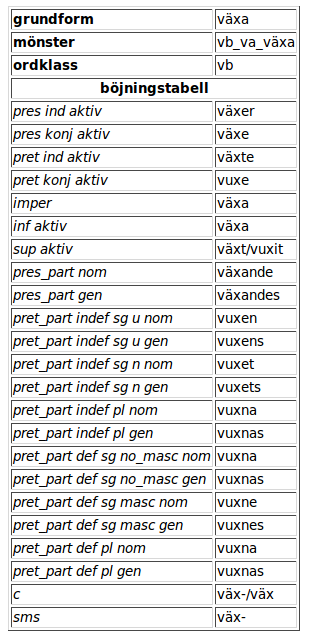
\includegraphics[height=90mm]{saldoVax.png}}
\hspace{5mm}
\subfloat[GF]{\label{pic:gfVax}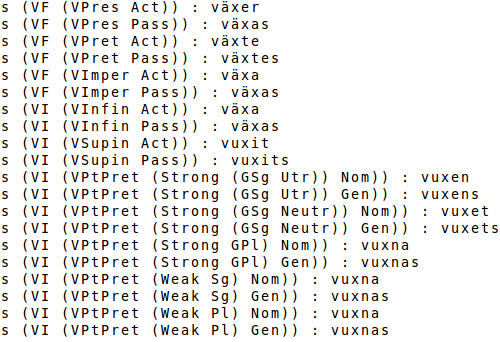
\includegraphics[height=60mm]{gfVax.png}}
\caption{Inflection table for the verb ``växa" (grow)}
\label{pic:TabVax}
  \end{center}
\end{figure}
The tables does not overlap completely, there are some more forms in Saldo's table (eg. the 
compounding form ``väx-")
while the one generated in GF contains some that are not in Saldo (eg. ``vuxits").
Saldo may also contain variats: ``växt" and ``vuxit" are both supine form.
As far as possible, the program makes up for this by only comparing the overlapping forms
and only requiring that GF generates one variant whenever alternatives are given. 
The program continues to generate new lexicons as long as there are more
paradigms to choose from and compare the results after each run.

The program has been made more robust than the previous version, it prints
logs and finally lists of the words that were not imported. The logs provides
information about which paradigms that were used for each word and the result
from comparing the inflection tables.
During the porting of Saldo, some renaming of the lemmas was needed.
Special characters like \emph{å,ä,ö} should not occur in GF function names.
Those are translated into \emph{aa,ae,oe} respectively. 
The Saldo identifier \verb|äta..vb| is thus turned into the GF identifier \verb|aeta_V|.
Since there might be two lemmas that share the same
identifier after the translation, a number is added to the name whenever a translation
have been done: 
\begin{tabular}{lll}
kältisk & $\rightarrow$ & kaeltisk\_1 \\
kaeltisk & $\rightarrow$ & kaeltisk \\
entrecôte &$\rightarrow$ & entrecoote\_1 \\ 
\end{tabular}

%Problems with naming convention, special
%characters (å,ä,ö,apostrop,entrecôte.) needs to be translated , but avoid
%classhes 'kaeltisk' 'kältisk', gf will crash by this, so we add a 1
%in the end whenever we have changed a letter.
%,é
%Costs very much memory, the saldo file is big, the generated lexicon is big.
%Saldo is divided to save memory. Errors should just be reported, but if something oförutsett
%happens and one part fail, the separation ensures that the others wont, also
%possible to restart. 

%Explanation of the algorithm: map categories, try each paradigm, compare the table of forms
%created. If several forms in saldo, gf should pick on of them. Saldo has forms for
%compounds, gf does not. A grammar is written, the correct ones saved, the others 
%retried. Try all paradigms which can be formed from saldo. 
%In Saldo there is also semantic info, so
%We need the numbers from saldo if there are to lemmas with the same
%identifier. växa (bli större), växa (vara en planta) vs. sluta\_V and sluta2\_V
%(slöt). However gf does not want more than one table
%if the forms are identical, saldo's morpho neither, but there are five in big saldo. 
%We are just interested in morphology, so far. Dont want too big lexicon.

%see notes to add more about this, pronouns and the importing itself
%choices for adjectives vs. verbs for particips
The importing can be redone anytime.

\section{Results}
All words from Saldo were not be imported. There are a number of reasons
for this, the most obvious one is that we do not want all categories from
Saldo in the GF lexicon. Prepositions(\emph{pp}) and numerals(\emph{nl}) etc.
~~are assumed to be known already~~,
and are usually not kept in the standard lexicon, but in modules for the basic
structures of the language. Categories involving several words(\emph{vbm,nnm})
need to be handled differently, usually as idioms. Pronouns(\emph{pn}) are not  
analysed the same way, see section \ref{sec:swegf}. Some experiments on finding
the right GF-category for those have been done, see ~~~~~\ref{sec:gf.quant}.
Six categories were imported: \\
>> english examples
\begin{tabular}{l|lll}
& Saldo tag & GF category & Example \\
\hline
 Adverb & \textbf{ab} &\textbf{Adv} & ofta \\
 Adjective&\textbf{av} &    \textbf{A} & gul\\
 Noun & \textbf{nn} &\textbf{N} & hus\\
 Verb & \textbf{vb} &\textbf{V} & springa\\
 Reflexive verbs  &\textbf{vbm}& \textbf{V} & raka sig\\
 Verbs with particles &\textbf{vbm}& \textbf{V}  &  piggna till\\
\end{tabular}\\

%
%There are a number of differences between and saldo Till skillnad från GF,
%saldo does not contain forms that aren't used gf generates all forms. A form
%needed to generate the gf table may not be given in saldo such as singular
%forms for 'byxor'. Also contains idioms, 'hålla huvudet kallt' and has
%different grammatical analyse, a lot of pronouns. Example. 
One reason for why words of the categories listed above could not be imported
is that Saldo does not contain information about ~~word forms that are not used~~.
In some cases those forms are needed by the smart paradigm. 
This was a common reason why nouns could not be imported. 
Consider for example
the plural tantum % \cite[44]{SAG}
noun ``glasögon" (``glasses"). Since the smart paradigm
requires a singular form, this lemma could not be added to the lexicon. ``Glasögon" could
be added manually, by using the ~~somewhat incorrect,annan betydelse~~ singular form ``glasöga" (``glass-eye").
The same problem occurred for verbs that always are used in passive form:
>> not passive!! deponent, s-verbs!!
``andas" (``breathe"), ``frodas" (``flourish"), ``lyckas" (``succeeed"). This
was the case for close to 80\% of the failing verbs of type \verb_vb_.

In some cases the smart paradigms could not generate the correct declination,
although this happened seldom. 
>> exapmles: % frysa,fisa passive preterium 

The resulting dictionary contains more than 100 000 entries, compared to the total size
of Saldo this is approximately 80\%. When testing the coverage of Talbanken,
we found that around 3000 words were still missing (excluding the one tagged as
numerals and proper names, but some names are still there). In addition, there were 1817 words
>> give reasons! should look good, not bad!
which were given different labels in GF than in Talbanken. Many of those are
acceptable, such as the ones in table \ref{tab:saldodiff} and reflects the difference 
made in the analyses, but others are examples of words that are still missing from
the lexicon.
\begin{figure}[h]
\begin{tabular}{lll}
Word & Talbanken tag & GF category \\
\hline
måste & MVPS          & VV \\
allting & POTP & N \\
få & POZP & Det \\
\end{tabular}
\caption{}
\label{tab:saldodiff}
\end{figure}
Among the words that were completely missing, more than 2000 was found to be nouns,
many of which were compounds, and this is hard because ...~~~

The lexicon does not contain any valency information since Saldo does not give any such
information. Valencies are however crucial for GF, and by using the results from the mapping
(see section \ref{sec:Mapping}) it should be possible to extract this information about this.
>> about what? how? strategy?
%The saddest thing: no valency info. Crucial for GF. Only reflexive and verbs with particles
%have any information. The earlier explained techniques may be used for this in Talbanken.
%To get even bigger material, use Korp, but then no guarantee.


\chapter{The grammar}
\label{sec:prog.grammar}
Although we can't expect to get a full coverage, we aim for a ~~high-quality~~
grammar with satisfactory coverage.
We have been developing a grammar fragment which have been adapted to cover
constructions used in Talbanken. The starting point has been the Swedish
resource grammar and the new grammar should still be compatible with this.
%A description of the Swedish implementation of the resource grammar is given
%in the next section, while
Before describing what has been added, will give a short introductions to the
the cats of resource grammar and the sw implementation in particular.
This is done in section \ref{sec:swegf} while section \ref{sec:Added} shows and
explains the development during this project.
%Explain what's in the resources, constructions present in most languages. 
%Been working on a grammar fragment based on Talbanken,
%like cool people like Montague. May also be interesting for other purposes.
%Swedish shares with Nor and Dan. Extra module, covering things like sw is a
%v2-lang, focusing parts of sentences. 


\section{The Swedish resource grammar}
>> start by easy examples, jag ser inte dig, du ser inte mig osv. 
>> plocka från svenska delen 1 2 4 
>> show simple trees
>> explain all in Sw. section.
>> show abstract and concrete tree, compare. (or in Gf sect)
>> no subjects or object, analyse is more from the lexicon,
>> compare to others, ask elisabet.
\label{sec:swegf}
The GF resource grammars contains a fundamental description of Swedish,
covering the morphology and many phrase and clause constructions. Most of the implementation
is shared with the other Scandinavian languages.
Apart form describing morphology, the resource grammar deals with
word order, agreement, tense, basic conjunction etc.

In figure \ref{fig:gftree1} we saw how the sentence ``Jag ser dig" is parsed.
Discuss questions, how are word order handled here? Maybe negation and anterior.
Let's look on how post-determination (sec ref) is implemented, we know that the
smart paradigms can handle the noun declination, now show 'katten' vs. 'den trötta katten'.
A N carries the inflection information, turned in to CN by setting number. Example, type
of N and CN. A CN may then be modified by APs, set field for this. When turned into NP, 
definitness is set, depends on the isMod -field. NP has case as a parameter.
\verb|DetNP : Det -> CN -> NP ; |
To turn in into a NP need to fix determination, by Det. Dets have .. fixed,
but allow variation in.. 
To form \emph{`fågeln'}, the determiner (DetQuant DefArt NumSg) is used.
Is a quantifier, hence does not require number, is given later.
%What is the difference?
In gf, only personal pronouns are considered to belong to PN. The rests (example from
saldo, which is pronoun in SAG as well) are either Quantifiers or Dets.
Once we have a NP, can use Predets. What they are.\\

For verbs, but also others, there is an important distinction for valency.
Encoded in the lexicon. Categories as V,V2,VS...
Either directly to VP if V, or needs to be given arguments. Can then add adverbs.
%Maybe talk about ställa.
Particles and prepositions, can't be seen on the trees. Can now see why the parse
trees are not complete. difference shows when fronting.
tycka om /tycka om -> om vad tycker du inte. fast bra
Swedish verb may have up to five arguments according to Stymne
'jag tar med mig den till Bo' : ta\_med\_V3 = dirV3 (reflV (partV (take\_V "med")) (mkPrep "till") ;
but is really 'till' part of verb?
VP is divided corresponding to satsschema (diderichsen) (renewed by SAG).
If the object is not given immediatly, the grammar uses slash.
"Speed up", instead of movement used slashes \cite{gazdar}.
Slashes good for question (vilken katt ser du idag)
relatives (katten som du tittar på) and topicalisation
The grammar has VP,Cl, SSlash, all missing NP.

Example, use variants {}.

>> change dot file to have VP NP in correct order
\enumsentence{\shortexnt{8}
{Har& han& inte& ätit& de & gula& äpplena& idag?}
{Has& he& not& eaten& the& yellow& apples& today?}} 
\label{gfSwe:parseable}
The grammar can construct and parse the sentence in example \ref{gfSwe:parseable}
and the parse tree is represented as in figure \ref{gfSwe:parsetree}.
%Covers sentences like
% better sentence where the verb phrase is split up?
\begin{figure}[h]
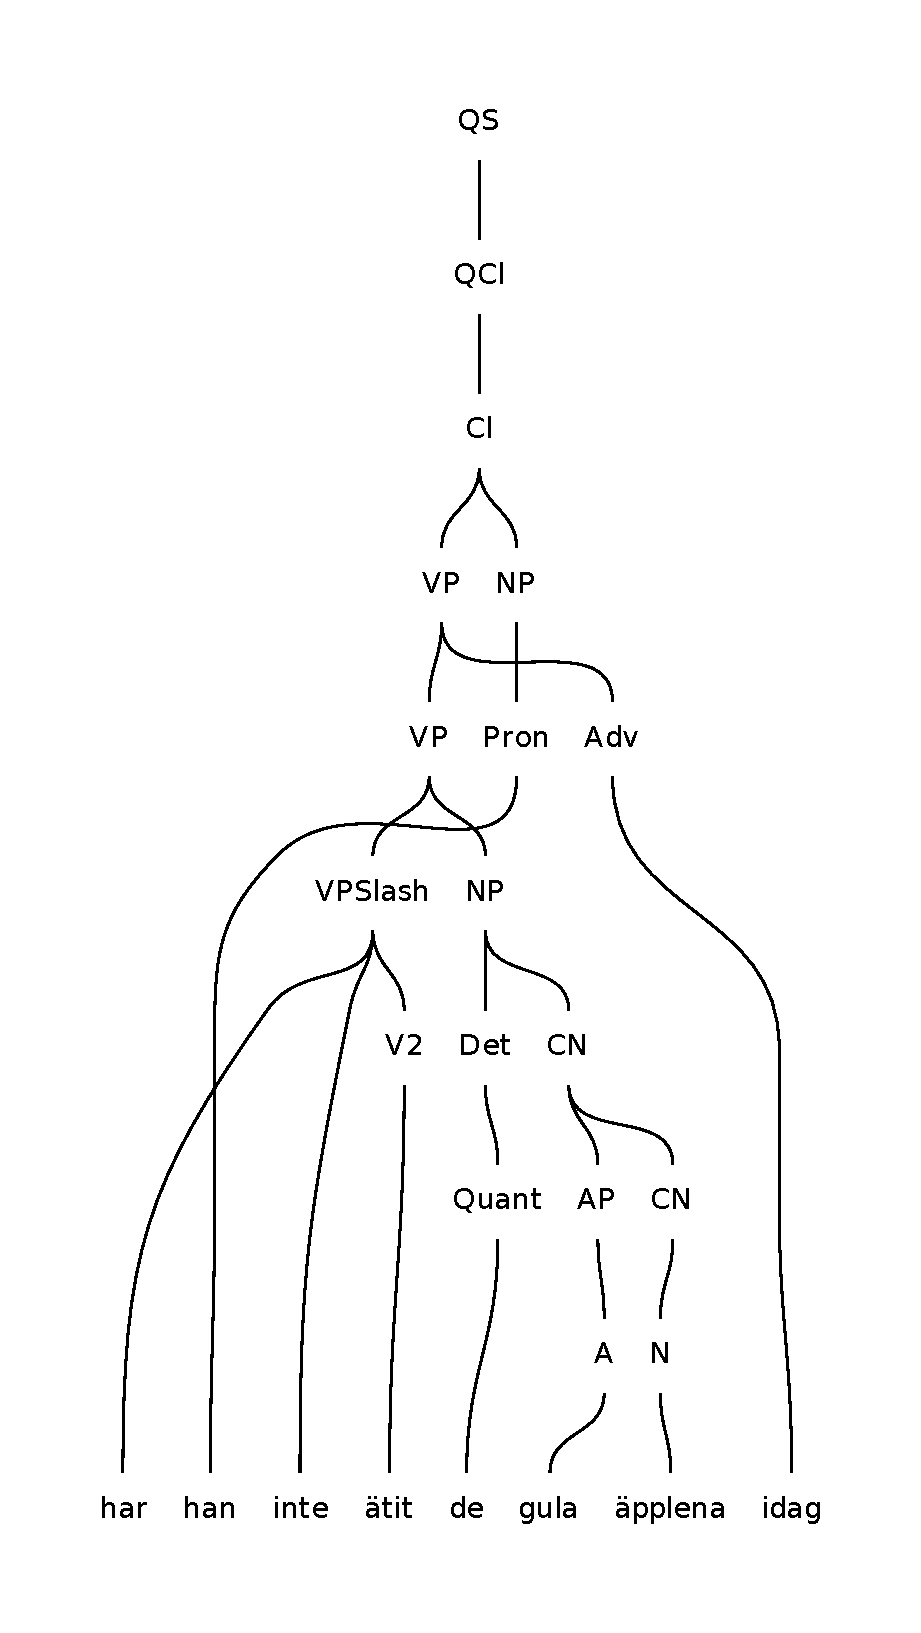
\includegraphics[width=70mm,height=70mm]{apples.pdf}
\caption{Parse tree for ``Har han inte ätit de gula äpplena idag".}
\label{gfSwe:parsetree}
\end{figure}
Even though the verb phrase \emph{``har inte ätit.."} is discontinuous, the whole
phrase is still treated as one constituent in GF. The parts
are connected in the tree, and the subject \emph{``han"} is put between the
finite verb and the rest of the phrase. At the code level, this is implemented
using records.
The linearization rule for questions -- clauses with inverted order -- picks 
the field for the finite verb and appends it to the subject followed by
the negation, infinite part and the complement of the verb phrase: \\
\verb|table { Inv => verb.fin ++ subj ++ verb.neg ++ verb.inf ++ verb.compl ; ... | \\

Relative clauses are also covered: 
\enumsentence{\shortexnt{5}{Hon & ser & pojken & som  &sover}
              {she & sees & the boy & who & sleeps}}
              %{`She sees the sleeping boy'}}

\enumsentence{\shortexnt{6}{Han & ser &katten & han  &tycker & om}
              {he & sees & the cat & he & likes &}}
              %{`She sees the sleeping boy'}}
In addition to the basic resource grammar, additional constructions had been added
to the module \verb|Extra|. The functions given here do not have to be translatable
to all other language, but are meant to cover language specific constructions.
%For example, the \verb|Extra| module included
Among those were functions for topicalisation, although not all
of them were implemented for Swedish.
%word order, agreement, tempus, adverbs, adjectivs...
%and relatives
%Also info in the Extra module, where more language specific constructions
%can be found.
For example, \verb|FocObj| fronted the object as in sentence \ref{gfSwe:apple}.
\enumsentence{\shortex{6}
{Det & äpplet & vill & jag & inte & ha}
{that & apple & want & I & not &}
{`I don't want that apple'}}\label{gfSwe:apple}
The module provided functions for preposition stranding:
\enumsentence{\begin{tabular}{ll}
Stranded preposition & cf.\\
Vem måste jag akta mig för? & För vem måste jag akta mig?\\
Who do I need to watch out for? & For whom do I need to watch out?\\
\end{tabular}}

%jag ser dig
%dig ser jag
%dig har jag inte sett
%jag har inte sett dig.
%how the parse tree is generated, the finite verb, the subject, the rest. usw.

%honom ville hon inte tänka på.



%What was in the resources
%description of the existing grammar, the types, the possibilities
%VP, NP.
%valency built in (problems with ställa - på, under, vid).
%Variants, nonexist.
%coverage of standard Swedish.

\section{Development of the grammar}
\label{sec:Added}
Summary of what have been added and motivation.

\subsection{A second future tense: ``Kommer att"}
kommer att - for scand, extra tense, example
example table

%%PASSIV
\subsubsection{Passive}
>> why not VPSlash here??
Passive voice is often used in Swedish, especially the
\textit{s-passive}.
\enumsentence{
\shortex{5}{Uppsatsen & skrev\textbf{s} & av & en & student.}
        {the essay & wrote+\textbf{s} & by & a & student}
        {`The essay was written by a student.'}}\label{sent:skrevs}
%{b. &En & student & skrev & uppsatsen.}
%        {&a &student &wrote &the essay}
%        {~~`A student wrote the essay.'}}
Some studies suggest that the s-passive is used in more than 80\% of the times \cite{laanemets}.
It is not as common in the other Scandinavian languages however, 
and it can not be used in all tenses for all words. The Norwegian 
translation of sentence \ref{sent:skrevs} is:
%The periphrastic passive is preferred, especially in spoken langauge.
\enumsentence{\begin{tabular}{ll}
Oppgaven ble skrevet av en student & [NO]\\
Uppsatsen blev skriven av en student& [SE]\\
\end{tabular}}
The corresponding Swedish sentence is acceptable, but not as natural sounding as sentence
\ref{sent:skrevs}.
The resource grammar for Scandinavian therefore ~~expressed~~ the passive using auxiliary verb. \\
>> change to:
\verb|PassV2 : V2  -> VP | \\
\verb|         ta -> blev tagen| \\
>> frånta, erbjuda works. add. check vp in urdu
>> how are they used with reflexives??
This rules allows two-place verbs to be used in passive by using \emph{bli} (\emph{become}), and thereby
turned into complete verb phrases; they no longer need an object.
The s-passive has now been added as the standard case for the Swedish GF
grammar. Periphrastic passive is still allowed, but as an alternative rather
than the default.
>> error!!! 
\verb|PassVPSlash : VPSlash  -> VP | \\
\verb|              ta -> togs| \\
\verb|              erbjöd -> erbjöds| \\
The grammar also allows not only V2 but all verb phrases missing an object to 
form passives:
\enumsentence{First place in two-place verbs\shortex{3}
{Jobbet & erbjöds & henne }
{the job & offered+\textbf{s}& henne}
{``The job was offered to her"}}
\label{ex:passV32}
\enumsentence{Second place in two-place verbs\shortex{3}
{Hon & erbjöds & jobbet}
{she & offered+\textbf{s}& the job}
{``She was offered the job"}}
\label{ex:passV33}
\enumsentence{\shortex{3}
{Huset & målades & rött}
{the house & painted+\textbf{s}& red}
{``The house was painted red"}}
\label{ex:passV2A}


%r
%\enumsentence{\shortex{6}
%{Betyget & 3 &ges &till &många &elever}
%{Grade & 3 & give+\textbf{s}& to & many & students}
%{``Grade 3 is given to many students"}}
%\label{ex:passV3}
%by letting the first object be `removed' and given by the subject. 
%
%A remark can be made about sentences where the second object is put first in the sentence, like 
%\enumsentence{Till många elever ges betyget 3}
%This is a variant of example \ref{ex:passV3}, \emph{`många elever'} is still the object but put in focus. The grammar
%parse this by applying \verb|FocObj|.
%%

%% Clauses
\subsubsection{Impersonal constructions}%Presentering, , Topicalisering
\label{sec:Formal}
Formal subjects \cite[19]{SAG} is often used in Swedish.
\enumsentence{\shortex{6}
{Det & sitter & en & fågel & på & taket}
{It & sits & a & bird & on & the roof}
{``There is a bird sitting on the roof''}}
\emph{`Det'} has the position of the subject, and the real subject, 
\emph{`en fågel'} the one of an object.
Transitive verbs may not be used like this
>> elisabet disagrees: use det äter en fågel ost på taket
\enumsentence{\shortexnt{6}
{*Det & gillar & en & fågel & på & taket}
{It & likes & a & bird & on & the roof"}}

unless their in passive form
\enumsentence{\shortex{5}
{Det&dricks&mycket & öl& nuförtiden}
{It&drink+s&much & beer& nowadays}
{A lot of beer is being drunk these days}}
A very common example of this is sentences with the verbs \emph{finnas},
\emph{saknas} and \emph{fattas}. > engelska.
\enumsentence{\shortex{3}
{Det & finns & kaffe}
{It & exist & coffee}
{''There is coffee"}}
\enumsentence{\shortex{3}
{Det & saknas&  kaffe}
{It & misses & coffee}
{''There is no coffee"}}
\enumsentence{\shortex{3}
{Det & fattas & kaffe}
{It & misses & coffee}
{''There is no coffee"}}

A special GF category, \verb|SimpleVP|, was needed for verb phrases of the type
described above.
>> read cooper and say smt smart here
There are also restrictions on the subject.
\enumsentence{\begin{tabular}{ll}
*Det sitter den fågeln på taket. & *Det sitter fågeln på taket.\\
``There are that bird sitting on the roof'' & ``There are the bird sitting on the roof'' \\
\end{tabular}}
The noun must be in indefinite form, even though some determiners are allowed.
\enumsentence{Det sitter några fåglar på taket\\
              ``There are some birds on the roof''}
\enumsentence{*Det sitter fåglarna på taket\\
``There are the birds on the roof''}
%%Quantifiers like \emph{`denna'} or determiners like \emph{`samtliga'} may
%%not be used, but the determiners \emph{`många'}, \emph{`några'} and the quantifier
%%\emph{`ingen'} work well.
%%Semantic difference, atm we allow any NP. \\
The GF grammar does not make any distinction between indefinite and definite noun
phrases. Therefore this is handled by looking at the determiner. \\
\verb|FormalSub : SimpleVP -> Det -> CN -> Cl ;|\\
The function combines a verb phrase a determiner and a noun phrase in to a clause.
If the determiner requires a noun in determined form, the clause is put to NONEXIST.
However, this is not an ideal solution. There are other examples of when we
need to know the definiteness of the noun phrase, for example when using
the reflexive possessive pronoun `sin' (see section `Reflexive pronouns' below)
or when using some predeterminers (see section `Quantifiers'). Not true, not the same :(

%finnas: här får man ha definit: det finns de som inte vill. Samma RelCl som
%jag just la till, de äppplen. (de + relsats)

%'det är kul att..' Näst vanligaste två-ordskombinationen i talad svenska.
%%
%embedded - relative, 'sådan att' not really nice for normal swedish, and no agreement
%between subject 'en katt sådan att det regnar'. Kan säga 'en sån katt som sover, med 'sådan' + Rel
%har lagt till Det äpple + Rel (RelCNNP). *Det äpple är rött. men Det äpple jag äter är rött.
% 


\subsubsection{Quantifiers, determiners and predeterminers}
\label{sec:gf.quant}
The GF analyse differs sometimes. Experiments of how to extract
this information from Talbanken by using Saldo as a starting point.
One of the biggest differences between the GF analysis and the one made in Talbanken
is related to pronouns. While GF only recognizes the personal pronouns, 
`sådan', `fler`, `somliga' etc. are all regarded as pronouns in Talbanken and Saldo.
In the GF analyse they may be quantifiers, determiners or predeterminers. 
All pronouns from Saldo was listed and by searching Talbanken for which tags
they got we could sort out the ones acting either as
determiners, as `sådana' in sentence \ref{ex:QuantDet}, or as adjectives as
`sådan' in sentence \ref{ex:QuantAdj}. 
\enumsentence{Sådana katter vill jag ha}\label{ex:QuantDet}
\vspace{-3mm}
\enumsentence{Han är sådan}\label{ex:QuantAdj}
\vspace{-3mm}
\enumsentence{Sådant är inte bra}\label{ex:QuantDet2}
Since all determiners can be used alone as noun phrases, sentence
\ref{ex:QuantDet2} is also accepted.
%what is the difference really???
%The techniques of searching Talbanken can be used
%for this purpose as well. 
%combining the information in Saldo and Talbanken
%pronouns/Quant. Many, created categories for 'sådan', and 'fler'. Not many in each,
%has to decide, one category for each?

\subsubsection{Other small things}

\textbf{Genitive} -problem 1 cannot be alone (fixed) 2 some words have id. (no) gen form (fixed)
           fixing this include restructuring all???
\textbf{Det-utr}. not effect for the some Dets, like 'sådan', no difference between utrum and neutrum.
 Can vary in number, since is a NP. Do not want to cut connection to abstract but changing them,
 so added one more. Leads to ambiguities in some cases, but considering that we would want to use
 this for translation, neutr and utr may differ in the other language.

\textbf{finiteness}
 'de flesta de gula hästarna'

\subsubsection{advs}
-- or is this really just AdVs? 
to change position of adv:
normal: after verb 'han äpplet redan'
now want: 'äter redan äpplet'
          'har redan ätit äpplet' 
          'har ätit redan äpplet' :( which doesn't work either :)
\subsubsection{Focusing adverbs}
GF separates between two categories of adverbs, the normal ones \verb-Adv-, 
eg. `nu' (\emph{`now'}) and
special ones (name!) \verb-AdV- like `alltid' (\emph{`always'}).
The \verb-AdV- attaches directly to the verb and have a special
field in the \verb-VP--table.
\enumsentence{\shortex{4}
{Jag & äter & aldrig & fisk}
{I & eat & never & fish}
{`I never eat fish'}}
\enumsentence{\shortex{4}
{Jag & äter & fisk& nu }
{I & eat & fish& now }
{`I eat fish now'}}

\begin{wrapfigure}{l}{0.3\textwidth}
\begin{tabular}{|l|}
\hline
bara \\
inte ens \\
till och med \\
\hline
\end{tabular}
\caption{Focusing adverbs}
\label{fig:focadv}
\end{wrapfigure}\\
The focusing adverbs, like `bara' (\emph{`only' or `just'}) may put in both? of this
positions and additionally, they may be used before the finite verb.


\enumsentence{\shortex{3}
{Han & bara & log }
{he & only & smiles }
{`He just smiles'}}

In order to implement this, a new field was needed in the \verb-VP--table,
which may be put before the finite verb.\\
\verb|s SPres Simul Pos Main : han bara sover|\\
compare to negation, \verb-AdV- and \verb-Adv-\\
\verb|s SPres Simul Neg Main : han bara sover inte alltid här|\\
example in Sub or Inv, 
When used together with modal verbs, the new field results in
some not very natural sounding constructions:\\
\verb|s SPres Anter Pos Main : han bara har sovit|\\
but rather than changing to 'han har bara sovit', we keep it. Is a possible
tolkning and the other case is covered by using it as an AdV, we don't want
ambiguities.

The foucusing adverbs may also be used as predeterminers:
\enumsentence{\shortex{7}
{Det & är & bara & barn & får & göra & så }
{it & is & only & childern & may & do & so }
{`Only children are allowed to do that'}}
This is handled by the rule:
\verb|PredetAdvF : AdvFoc -> Predet ;|

\textbf{antalet}
Also needed categories for 'pronouns' which can act in different ways.
and 'antal','sorter' - need indetermined, antal plural, sorter either.
Should be able to modify by a arbitrary antal adjective, and they must be determined.
'(ett stort antal) människor' and not 'ett stort (antal människor)'
Don't want them as a NPs or CNs since we don't want other Ns to be used this way
'en flicka kaffe', this is then Appos? (Or do we?). Should also not be utsatta for what other
NPs or CN can be. Dessutom, we want to make use of the comp-fiel. 'mamma till', but is this really
the same??

\textbf{VP}
The VP require many changes PPart, bara.
About PPart, but do we need it with new Saldo? 'de är stuckna' , 'den nyligen funna'
for the last one, we need VPSlash to allow adverb.

\textbf{SuperlA}

In general, many categories need more parameters and fields, tex Quant can be used as NP
and therefor needs to depend on Case, de -> dem.

here or in robust: SupCl, det as VP or VV or S for S (remember Foc)
\subsubsection{Reflexive pronouns}
%varandra and sin/sitt/sig.
An important piece in a Swedish grammar is the reflexive pronouns and
%both \emph{sin} and , eg. \emph{sin}.
the possessive pronouns as described in section \ref{swe:refl}.
Those make up noun phrases which are not allowed in subjects, 
and we want to be able to parse to following sentences:

>> remove stupid examples, add 'hon och sin vän åkte tåg'
>> use self instead of his.
\enumsentence{Han såg sina barns skor.\\ \label{ex:ReflGen}
He saw his children's shoes.}
\enumsentence{Sina vantar hade han glömt på tåget.\\
His gloves, he had forgotten on the train.}
\enumsentence{Han ger sina pengar till sina syskon.\\
He gives his money to his children.}
\enumsentence{Han är längre än sin kompis.\\
He is taller than his friend.} \label{ex:ReflAP}
\vspace{-2mm}
\enumsentence{Han är här oftare än sin kompis.\\
He is here more often than his friend.} \label{ex:ReflAdv}
\vspace{-2mm}
\enumsentence{Hon tyckte om skolan och alla sina elever.\\
She liked the school and all her students.}\label{ex:ReflConj}
\enumsentence{Han såg sina få böcker och sin penna.\\
He saw his few books and his pencil.}\label{ex:ReflConj2}
\vspace{-2mm}
\enumsentence{Hon ber alla sina kompisar att gå\\
She asks all her friends to leave}\label{ex:ReflPredet}
\enumsentence{Jag vill att han rakar sig.\\
I want him to shave.}
but not
\enumsentence{*Sina vantar var kvar på tåget.\\
Her gloves were left on the train.}\label{ex:ReflSubj}
\enumsentence{*Jag ger sina pengar till sina syskon.\\
I give his money to his siblings. }
\enumsentence{*Han vill att jag rakar sig.\\
He wants me to shave himself.}

The reflexive pronouns require an antecedent with which they agree in
number and person. Apart from this restriction, they may be used as normal
noun phrases and ~~conjuncted~~ (sentence \ref{ex:ReflConj} and \ref{ex:ReflConj2}),
determined (sentence \ref{ex:ReflPredet}) and used as genitives (sentence
\ref{ex:ReflGen}) as such.
%Could be combined with 'sig', a ReflNP without another noun.
In short, what is wanted can be summarized as follows:
\begin{figure}
\begin{enumerate}
\item{
Construct a noun phrase from a common noun phrase \\
katt $\rightarrow$ sin katt} % \\
\item{Modify it like a \verb|NP|\\
sina katter $\rightarrow$ alla sina katter}
\item{Use it only as object\\
sin katt $\rightarrow$ han såg sin katt }
\end{enumerate}
\caption{Rules for noun phrases with reflexive possessive pronouns}
\label{fig:reflrestrict}
\end{figure}
If we ignore the second requirement, special functions for using common nouns
together with reflexive possessive pronouns could be introduced:
\begin{verbatim}
ReflVP: CN -> VPSlash -> VP ;
        mat + äta     -> äta sin mat 
\end{verbatim}
This way, using the phrases as subject is excluded, but neither of sentence
\ref{ex:ReflConj}, \ref{ex:ReflConj2} or \ref{ex:ReflPredet} is allowed.\\
The simplest way of fixing this is to treat the phrases as normal \verb_NP_s.
We can add a rule for using the possessives with common noun phrases:
\begin{verbatim}
ReflNP: CN -> NP ;
        mat -> sin mat 
PredetNP : Predet -> NP       -> NP ;
           alla   + sina barn -> alla sina barn
\end{verbatim}
But by keeping them as \verb_NP_s we lose information, and there is no way of
keeping them from being used as subjects. We have ignored the third restriction
and are allowing sentences like \ref{ex:ReflSubj}.

Another solution introduces a new object type, \verb_Obj_, which is
identical to normal \verb_NP_ except for that it depends on 
the antecedent. All functions using noun phrase as objects are changed to dealing
with objects instead.
\begin{verbatim}
ReflVP: Obj     -> VPSlash -> VP ;
     -- sin mat +  äta     -> äta sin mat 
NPtoObj : NP  -> Obj ;
PredVP  : NP -> VP -> Cl ;  -- NP used as subject
\end{verbatim}
Any normal noun phrase may also be used as an object, whereas subjects only
can be made up by \verb-NP-s.
Since the resource grammar did not make any distinction between
subjects and objects, the new Swedish grammar needed to be separated from the old
structure. 
Further, the dependence on the subject needs to be applied to adverbial phrases and
adjective phrases as well. The adjective phrase in sentence \ref{ex:ReflAP} and
the adverbial phrase in sentence \ref{ex:ReflAdv} are examples of this; if the
subject was changed to 2nd person, they  would need to change too.
\enumsentence{\textbf{Du} är längre än \textbf{din} kompis.\\
You are taller than your friend.} \label{ex:ReflAP2}
\vspace{-2mm}
\enumsentence{*Du är här oftare än sin kompis.\\
You are here more often than his friend.} \label{ex:ReflAdv2}
Adverbial phrases may also be parts of new noun phrases
\enumsentence{\shortex{3}
{Taket & på sitt hus &}
{\scriptsize{\textbf{NP +}} & \scriptsize{\textbf{(Adv with Obj)}} & $\Rightarrow$ \scriptsize{\textbf{Obj}} }
{The roof of his house}}
\enumsentence{\shortex{3}
{Sitt hus & på berget &}
{\scriptsize{\textbf{Obj +}} & \scriptsize{\textbf{Adv}} & $\Rightarrow$ \scriptsize{\textbf{Obj}} }
{His house on the mountain}}

The first restriction in figure \ref{fig:reflrestrict} should be slightly
modified, to allow certain kind of \verb|NP|s to be used.
\begin{figure}[h]
\begin{enumerate}
\item{
Construct a noun phrase from a common noun phrase or certain noun phrases \\
få katter $\rightarrow$ sina få katter} 
\end{enumerate}
\caption{Modification of \ref{fig:reflrestrict}}
\end{figure}

The kind of noun phrases that can be used seems to coincide with the ones
that can be used with formal subjects (see section `Impersonal constructions').
>> subject controlling verbs
>> why comlicated with doubled types, show simplicity (elegant) with dep.types, and
>> some problems (many fields).
>> samesame as Obj, but conjunction works too, sin is Quant but what i sig?
>> (show circle (sig : NP -> GenNP sig -> sin??)
>> how we can add dependent type for Num to use 'varandra'
>> CN should have dettyp too, 'avståndet till sin bil'

>>Mention varandra. Same idea.
>>agreement to subj: Also good for double functions : Flickan, hon var inte dum, hon?
% F1,2,3 : NP -> VP -> Cl ; NP needs gender (Masc,Fem,Utr,Neutr)


%Make a distinction between objects and subjects?
%do not want to copy all rules for another category. Would like depent types!
%work pretty well by letting all NP depend on the subject in the phrase.
%The current version is nice and works for recursive genitivs!
%Extra info, but maybe this is just the case about NPs.
%Discuss how other solutions, NPR and Predet : Predet -> CN -> NPR ;
%*Slash* : VPSlash -> NPR -> VP ;
%Keep number of fields down, but introduces another category, and one more
%label to the parse tree, is it interesting? How to combine it with genitive 
%without making it ambiguous (Han såg barnens hund).
%What if we add alot of other rules that uses NP, will they all need to be
%duplicated then?

%'han såg sin mammas bil', they same could be applied to
%APs for example \ref{ex:ReflAP} or Adv for
%\enumsentence{Han leker oftare än sin kompis}
% (ComparAdvAdj)
%Atm you can't focus this kind of object, then a ClSlash need info about the
%subject. FunRP also tricky (and what does it mean, we can say
%Han såg sin katt i vilken musen låg), in this case RP needs to give more information.
%Kort sagt, the information about the subject must be spread
%in different parts of the sentence. 
%Could also decide to always produc 'sin' -> jag såg sin bil
%to avoid the dependence, but not nice. Or keep a flag in NP saying if it is
%in third person, and add nonexist for others. But this way we can also get rid
%of ReflVP and the possessive prons \verb|PossPron| should only be used for somebody else:
%'jag såg din bil'.
%Unfortunaly, have to change ReflVP, this only allows this in object for VPSlash, not FocObj,
%not 'alla sina', usw. Want it to handle conjuction as in example \ref{ex:refGen}
%etc.
%varandra, works the same but has no case for Sg.
%%

\subsubsection{Relative clauses}
The resource grammar already provided a number of ways to express relative and embedded clauses, such as
\enumsentence{Frågan är vilken färg den har\\
                   Pojken, som är blyg, tystnar\\
                   Han såg kunden som tyckte om sallad\\
                   Jag tänkte på huset i vilket hon bodde} % better example!!

A few problematic things can be illuminated:
Since the constructions are inspired by other languages, some of them may sound quite
non-natural in Swedish, such as the \verb|RelS|. This combines a sentence \emph{`Hon sover'}
and a relative sentence \emph{`som/vilket är bra'} which wrongly expressed 
\emph{`She sleeps, which is good'} as
\emph{`Hon sover som är bra'}. The error comes from the fact that \emph{`som'} is
embedded in the relative clause. This is easily fixed, by adding an extra
parameter was needed to tell whether \emph{`som'} or \emph{`vilket'} should be used. \\
Another complication stems from \verb|RelCl| which express the english \emph{`such that'}.
The Swedish version \emph{`sådan att'} sounds stelbent, when used outside of logic books.
\enumsentence{Jag vill ha en katt sådan att den inte fäller.} 
This relative clause in the sentence is, in GF, put together by two constituents: \emph{`` katt"}
of type \verb-CN- and \emph{``den inte fäller} of type \verb-RCl- (relative clause). They are
glued together by \emph{``sådan att"} and \emph{``katt"} should agree with \emph{``den"}. 
\enumsentence{*Jag vill ha en katt sådan att \textbf{det} inte fäller.} \label{sent:detfaller}
However, this is not the case and sentence \ref{sent:detfaller} is currently
accepted by the grammar.

The grammar has been extended to accept
\enumsentence{\shortex{7}
{\textbf{De uppfattningar}& som& förs& fram ...} 
{The opinions& that& put & forward ...}
{``The opinions presented ..."}}
where \emph{``de"} is used together with a indefinite noun. This is only correct for 
relative clauses or together with the verb \emph{``finnas"}.
In other cases definitev form must be used, cf. sentence \ref{sent:debocker}.
\enumsentence{\textbf{De uppfattningarna} förs fram.\\
``The opinions are presented."}\label{sent:debocker}
% also ok in finnas!!

%An more natural sounding alternative would be
%\enumsentence{Jag vill ha en sådan katt som inte fäller.}
%and hopefully this will be implemented soon, otherwise: why is it hard and how we can say
%'en katt sådan att det regnar'. It is relative but has on empty field, still congruation is
%needed.
%du är här, vilket jag vet.
%i de äpplen/det äpple du äter bor en mask/ som du ser.\\

\section{Testing}
Hard do test, can't verify. Regression testing. Talbanken is still too hard.
While developing: regression, 150 sentences to start with. Made longer, both good and bad,
to see how many ways things can be parsed.
Test how many parse trees that are generated.
Look at tables for a VP tex.
Some results.

% One part about the grammar. The state of the original grammar, what was covered and not. 
% What parts that I have been working on and why, 
% what constructions I wanted to add, examples of sentences that should work
% and of sentences that shouldn't be covered. How to separate Swedish from
% Scandinavian, bigger reconstructions in the grammar. 
% sammanhängande explanation of the swedish grammar, choices I have made, why
% regression testing

\chapter{Mapping}
>> no subjects or object, analyse is more from the lexicon,
>> compare to others, ask elisabet.
>> diffs: valencies, pp (gf ingen skillnad direkt/indirekt i träd, pga multiling)
>> mamba very used and tested for swedish, standard.
>> focus on what we DO cover.
\label{sec:Mapping}
Talbanken contains much valuable information about phrase structures and word 
usage. It is analysed with the MAMBA annotation scheme (Telemann, 1974) which is 
%>> cite mamba? annotation: well intergrated in sw. tradition, descriptive, used
%>> for large scale projects.
%annotation scheme
commonly used, and hence very well-tested, for describing Swedish.
The deepened analyse in Talbanken05 includes the lexical MAMBA layer. 
One part of this project has focused translating trees from Talbanken to GF.
We hence get a comparision between the two annotaitons and at the same time
we get ways to extract and translate information to GF notation. We have
constructed a mapping, which 
automatically transforms trees in Talbanken format to GF abstract syntax trees.
Figure \ref{fig:translationtrees} shows an example of a visualized Talbanken05 tree
of the sentence \emph{``The cat on the car gets bigger"} and the result of translating it to GF.
During the translation all the information given in the abstract tree
(\ref{pic:gftree}) needs to be extracted. We need to know that \emph{``katten"} is a noun
used in definite form (\verb-DetArt-), singular (\verb-NumSg-). Even though the
notation is changed by the transformation, the original analyse from Talbanken,
that ``på bilen" forms a subtree which is attatched to ``katten" for example,
is preserved.
%produces a \verb-NP- from ``katten" this means that
%DetCN : Quant                  -> CN    -> NP
%DetCN  (DetQuant DefArt NumSg)    cat_N = katten
Both the POS tags as well as the syntactic information are needed.

\begin{figure}[h]
\hspace{-10mm}
\subfloat[Talbanken tree]{\label{pic:tbtree}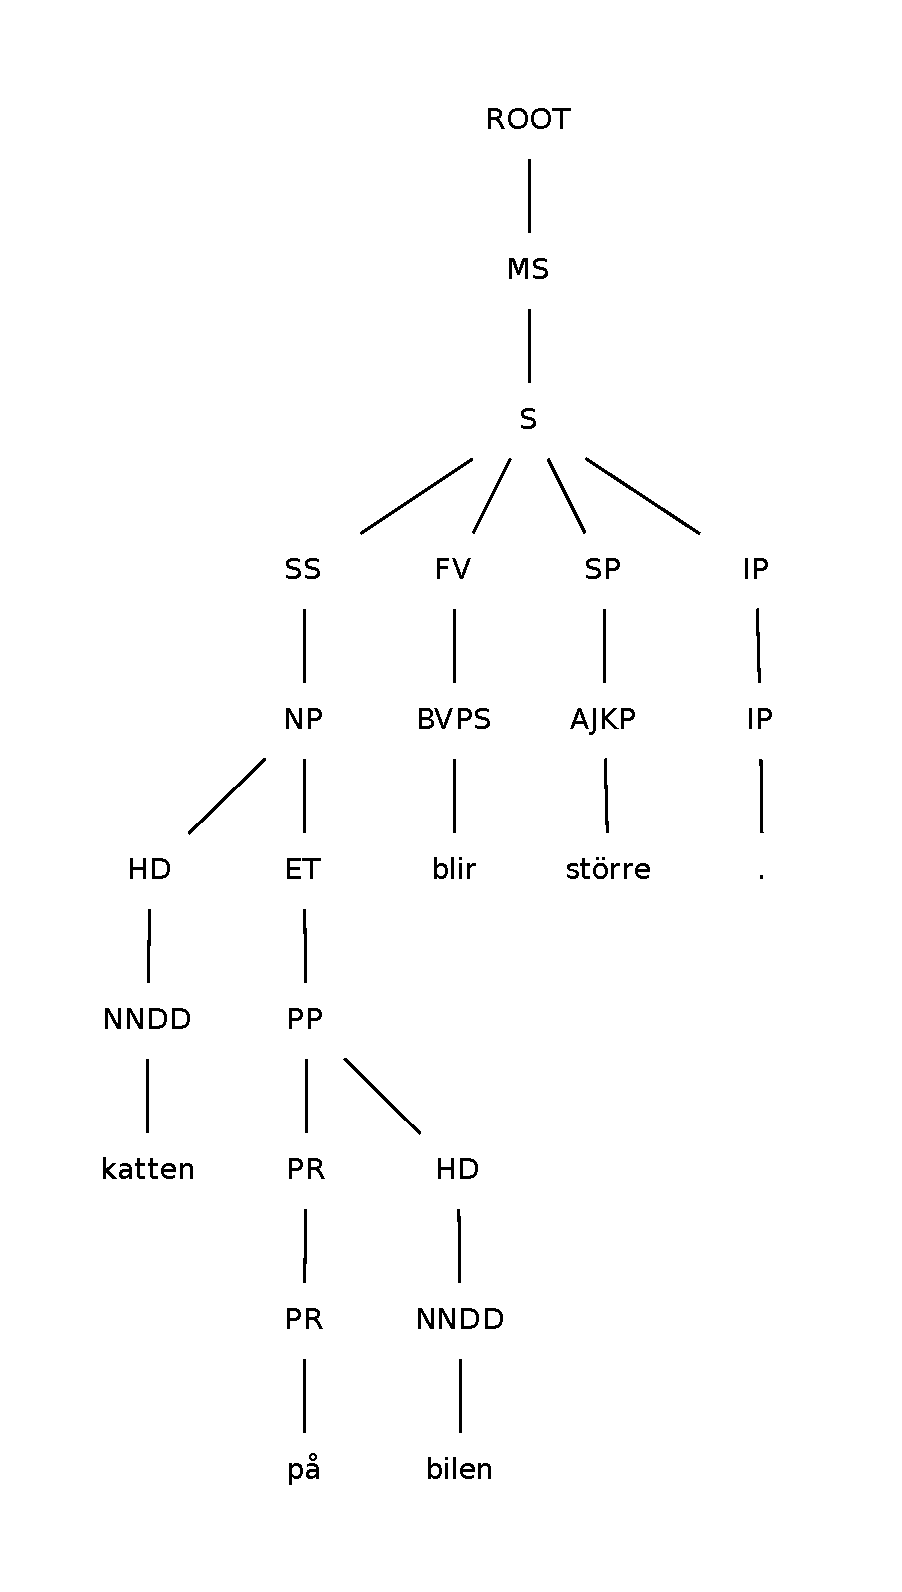
\includegraphics[width=60mm]{Talbankentree.pdf}}
\subfloat[GF abstract tree]{\label{pic:gftree}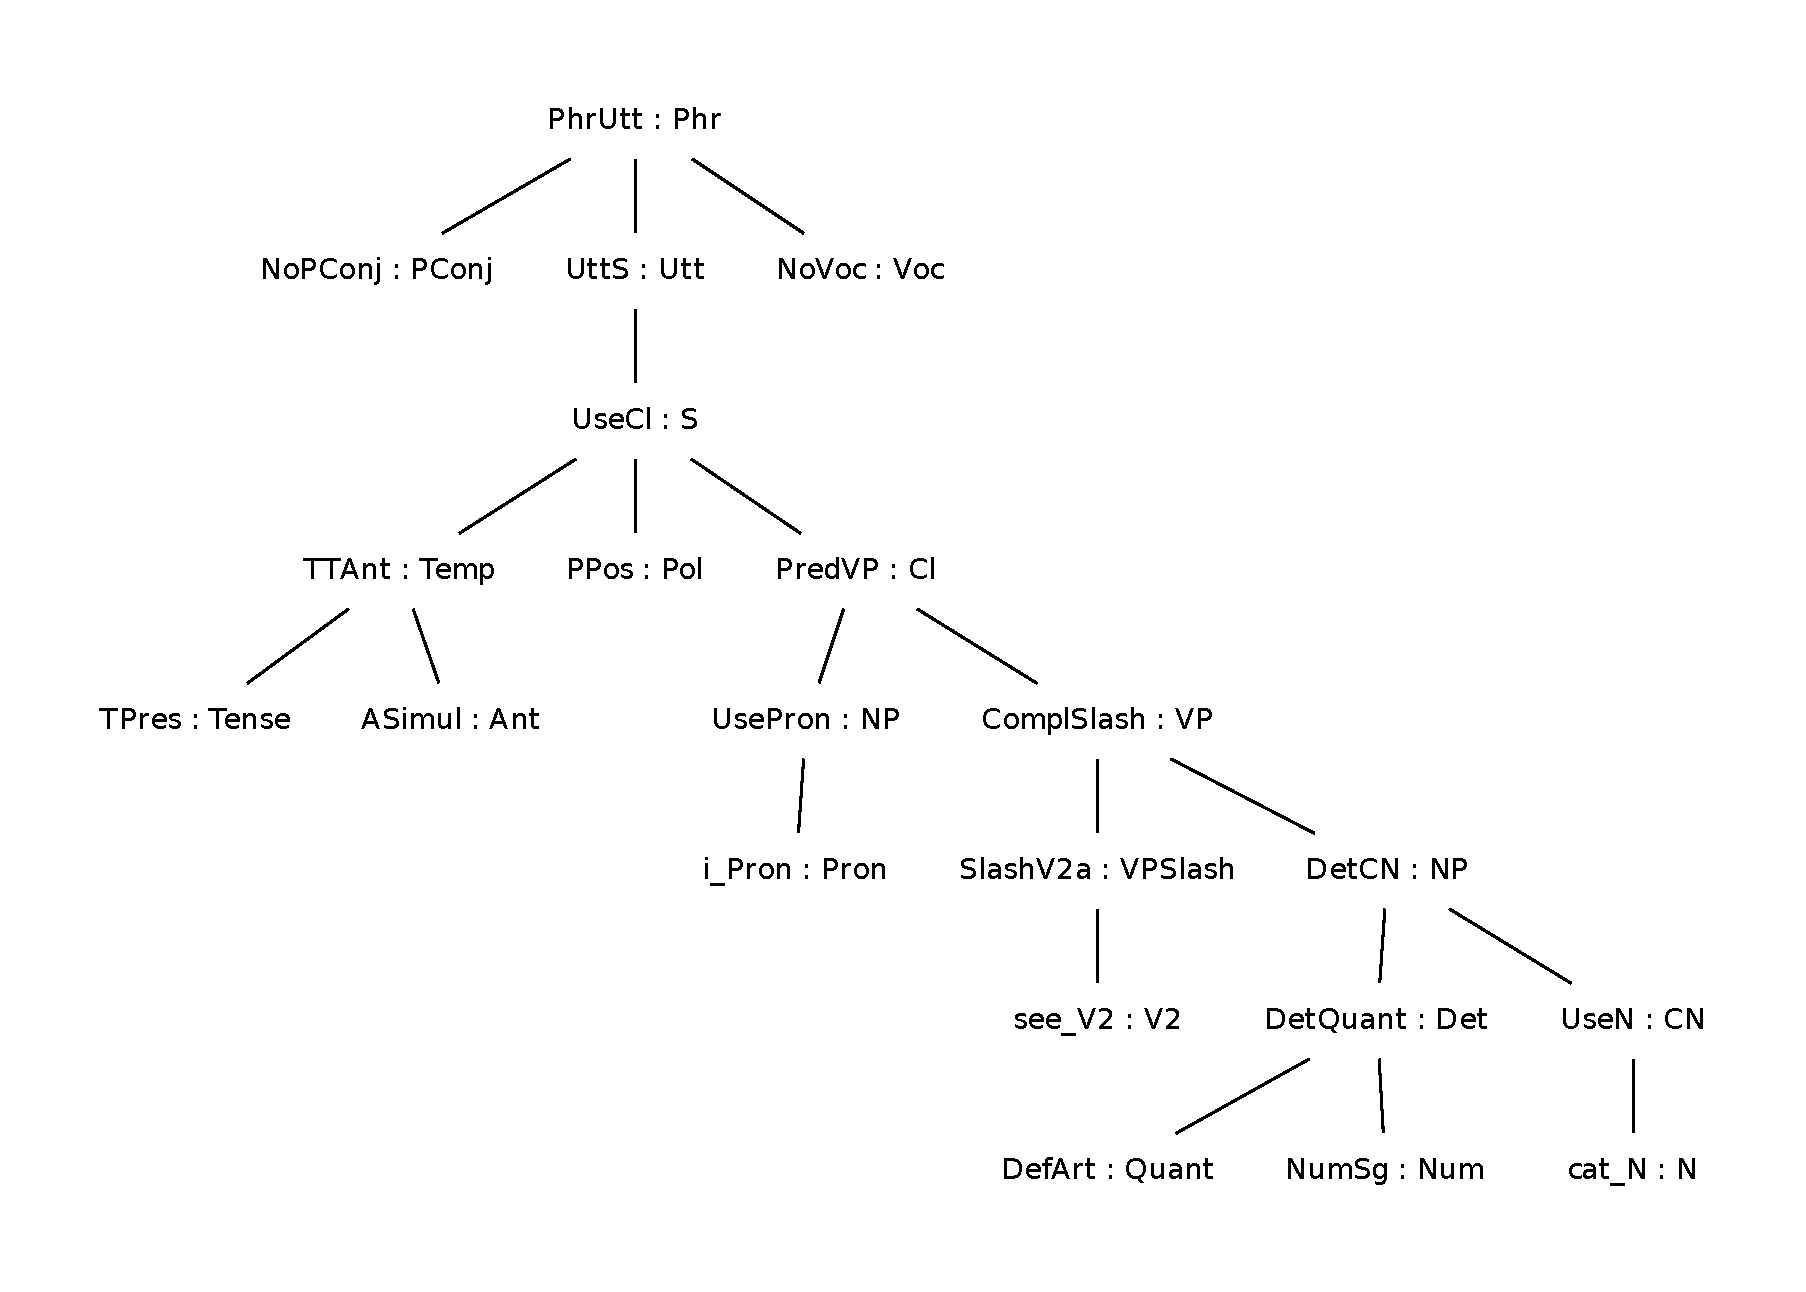
\includegraphics[width=60mm]{gfTree.pdf}}
\subfloat[GF parse tree]{\label{pic:gfptree}\includegraphics[width=50mm]{gfPTree.pdf}}
\caption{Trees for the sentence ``Katten på bilen blir större".}
\label{fig:translationtrees}
\end{figure}

The mapping connects GF with another annotations and gives us means to evaluate
our parser. By both parsing a Talbanken sentence and transforming its annotated tree, we can
easily inspect if the results are equal.
The mapping also makes it clear which grammatical constructions that are still missing
from the GF grammar and shows how the GF analysis differs from the one made
in Talbanken.
If there are words missing from our dictionary, the rich
POS-tags may help us to automatically find the correct declination and add it to the
lexicon. Further, our parser will need probabilities, see section
\ref{sec:future}, of how often a function is used.\\
%missing words. Lexical aquisation, probabilities, see section .
%The mapping gives information about which form a word is
%currently used in and this may be used by the lexical extraction
%tools. % Those can be enhanced if they are given more data. 
%The translated trees enable us to extract those probabilities. %The mapping gives us a source for this.
%Furthermore, the translation makes it easy to identify grammatical constructions
%missing from the GF grammar Another important use of the mapping is evaluation of the parser, which can be
%accomplished by comparing the parse trees and the trees from the transformer.

A translation of the English Penn Treebank to the GF syntax has previously been done \cite{gfpenn}.
By starting this from program, we now have
a translation that works for the differently annotated Talbanken. The differences between
Swedish and English syntax also meant that many rules had to be changed.\\

The mapping works for Talbanken05 in Tiger XML-format.
There are three kinds of tags: categories, edge labels and POS tags. 
The categories give syntactic information such as \verb|S|, \verb|NP| and \verb|VP|.
The edge labels give similar information with tags as \verb|SS| for subject, 
\verb|OO| for object. There are more than 300 different pos tags. The high
number is due to the detailedness, for example there are almost 50 tags for
nouns, excluding proper names. The tags show definiteness, case, whether the
word is a compound. Some words also have their own tags.\\

\begin{tabular}{lll}
\textbf{Tag} & \textbf{Example} & \textbf{Explanation} \\
\hline
\textbf{SV} & ska & The verb \emph{shall}\\
\textbf{WVIV} & vilja & The verb \emph{want} in infinitive\\
\textbf{KVSP} & kommit att & The verb \emph{will} in supine\\
\textbf{GVPT  PA} & gjordes & The verb \emph{do, make}, present, passive \\
\textbf{NNDDHSGG} & familjemedlemmarnas & Noun, definite, compound (person), genitive \\
\textbf{PU} & * \; 1) \; a) & List item\\
\end{tabular}\\

%Pos continues
%to either new tree or a word. Example S -> PP -> (Hd -> Id , Hd -> Id). Show
%corresponding GF tree.

The translation works section-wise, ie. if it finds a tree of category \verb|S|,
it will start to look for a subject \verb|SS| and a finite verb \verb|FV|. If it
can find those, they can be combine with the GF function \verb|PredVP|.
At the lowest level in the tree we look up the word in the GF lexicon.
It figure \ref{pic:tbtree}, the verb is followed by an adjective as a present
participle, \verb|SP|. GF admits \emph{``bli"} to have type \verb|VA|, a verb
with an adjective as complement, and the translator can apply the GF function
\verb|ComplVA| to combine the verb with its object. \\
It is not always the case that we first find the subject, then the verb and 
finally the objects. Often the order is Verb-Subject-Object or Object-Subject-Verb. \\
During the mapping process, the translator also needs to find out whether the sentence is
negated and what tense is used. If it finds two trees of type, say, \verb|VP| but does not
have any rules for combining them, the \textit{meta function} \verb-?- will be used. 
Figure xx shows an example of this.\\

%How we try to build up a 'abstract syntax tree', a S with a NP VP for example. 
%Continue with dividing VP into Verb Objs. More possible word orders (or at
%least more commonly used). 'katten åt sin mat fort' 'åt katten sin mat fort' 'sin mat åt katten fort'
% If can't find, add a '?', a meta.
%This is also what happens when the translator finds a combination it doesn't know about.
%Example of tree with meta.

%Description of most important tags from Talbanken, their translation? appendix?
\subsubsection{Differences in the notation}
Some structural differences between GF and Talbanken were made obvious during the
translation. \\
%Since the translation is done word by word, ambiguities may confuse the translator.\\
%shown during the translation.
%cause some translation problems.
In Talbanken the valency information is given implicitly by the complements
of a word. If a verb is followed by an object, \verb-OO-, which contains a
\verb-S-, we can conclude that this is a sentence-complemnt verb.
In GF, the valency information is given for each entry in the lexicon.
A sentence-complement verb has the type \verb-VS- and from this we know 
that the function \verb-ComplVS- should be used to combine the verb and with a 
sentence.
A similar issue arises form the use of verb particles. A verb with a
particle is considered as one constituent in GF, which means that the particle
has no effect on the abstract tree. Its presence is announced by the verb
itself, while Talbanken treats them as separated units.
%In Talbanken, verbs and particles are treated as separate units,
%and the particle is marked with the tag \verb-PL- and attached to. 
%Talbanken has no valence information while this is crucial for GF.
%The grammar requires a adjective-complement verb,
%\verb|VA|, to be used with one adjectival phrase. For \emph{``bli"} in example
%\ref{pic:tbtree}, we know that we need to find an adjective phrase.
%%know what kind of verb we are looking for
%%when consulting the GF lexicon.
%If the GF lexicon assings different types to verb, the correct type 
%should be showed by the complements.
%This way %\enumsentence{Han gillar det\\He likes it} 
The mapping cannot depend on the valencies given in GF only, however, 
since the distinction between different types of verbs is not always clear in Swedish.
The grammar rules becomes too strict for accepting most Talbanken sentences.
For example, most transitive verbs can also be used as intransitive. Both sentences in
example \ref{ex:mappTransitive} are grammatically correct.
\enumsentence{
\shortexm{11}
{Han& sitter& och &läser.}
{He& sits& and &reads.}{}
{Han& sitter& och& läser& en& bok.}
{He& sits& and& reads& a& book.}{}}
\label{ex:mappTransitive}
See section \ref{sec:futureValency} for a longer discussion about this.\\
%the Talbankenwill allow words to be used in other ways than their
%GF valencies prescribes.
Another problem can be illustrated by sentence \ref{ex:mappMan}, containing
the generic pronoun \emph{``man"}.
\enumsentence{
\shortex{3}{Man & uppskattar & dem}
{One & appreciates & them}
{``They are appreciated"}}\label{ex:mappMan} %  (s216).
In Talbanken, \emph{``man"} is simply a personal pronoun, 
in GF it is represented by using the function \verb|GenericCl|, which 
turns a \verb-VP- into a clause and has no
subject visible in the abstract tree. See figure \ref{fig:mappMan}.
\begin{figure}[h]
\centering
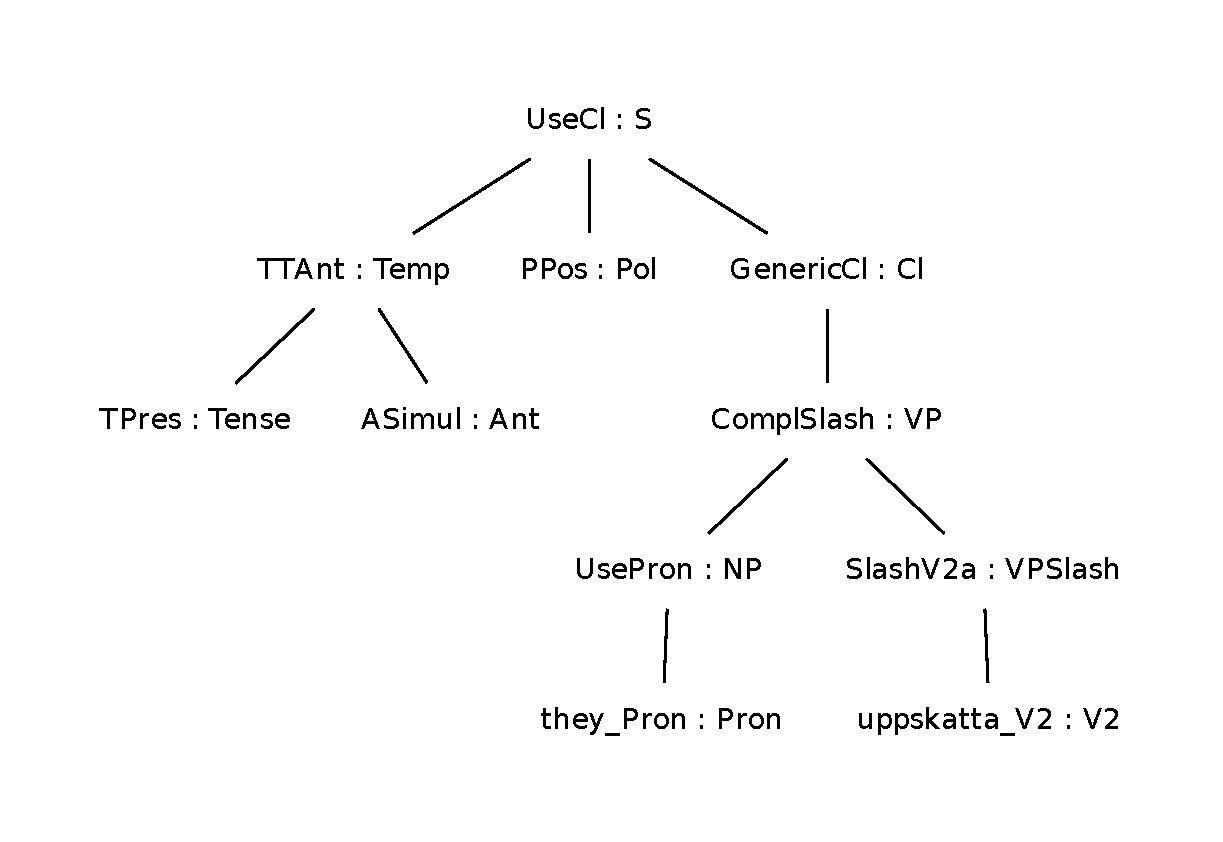
\includegraphics[width=80mm]{man.pdf}
\caption{Abstract tree for ``Man uppskattar dem".}
\label{fig:mappMan}
\end{figure}
When translating a senctence like this, it is thus not possible to simply glue the
subject to the verb with \verb|PredVP|.\\
%Therefore, the translator must change the type of the 
%sentence when inside the SS.

%The lexicon may contain a verb both with and without a particle,
%for example \emph{tänka} (``think") and \emph{tänka till} (``consider").
%\begin{verbatim}
%taenka_V  : V ;
%taenka_till_V : V ;
%\end{verbatim}
%When the translator looks up a the form \emph{tänka}, both of the two verbs
%will be among the results. %It is not known until later which one 
%%The first option will be selected, and if the
%%particle isn't directly attached to the verb
%%There is, at this point, no easy way of knowing which one of them wants a particle and the
%the transformation might confuse the two words. This is also the case when translating
%all sorts of idioms that GF considers to be just one bit.\\
%
%Difficulties in looking up 'idioms' like this
%in the gf lexicon. Therefore the translator might get confused.
%Sentences are also differntly deep. Example of a conjuncted sentence.

One of the reasons why \textit{metas} are put in the output, is the 
use of the tags show in table \ref{fig:mapBadtag}.
\begin{figure}[h]
\begin{tabular}{ll}
\textbf{NAC} & Not a constituent\\
\textbf{XP} & Other (non-coordinated) phrase\\
\textbf{DB} & Doubled function\\
\textbf{PU} & List item\\
\textbf{XX} & Unclassifiable part-of-speech\\
\end{tabular}
\caption{}\label{fig:mapBadtag}
\end{figure}
The analyse in Talbanken makes a difference between subjects
and objects, which is not needed in GF (see section \ref{sec:swegf}).
Senctences like
\enumsentence{För stora krav.\\
``Too high demands."}
hence makes use of the tags \textbf{XX} and \textbf{NP}, since it is not obvious whether
the noun phrase is used as subject or an object.
The tags shown above occur quite frequently in the treebank and are always translated
to metas. 
%How we cannot cover all cases. 

\section{Results and evaluation}
>> more! replace words, how much better results (both grammar and mapping) 
>> more results
>> motivation, why so bad??
The flat version of Talbanken05 was used for developing the mapping, but
the program works for both versions.
The deeper contains six more tags, but they are not always useful for our       
purpose. Figure \ref{fig:mappDeepFlat} shows the difference for a conjunction.
% show piece of s5 here!
\begin{figure}[h]
\centering
\subfloat[Deep]{\label{pic:mappDeep}
\includegraphics[width=20mm]{nofile.png}}
\subfloat[Flat]{\label{pic:mappFlat}
\includegraphics[width=20mm]{nofile.png}}
\caption{...}
\label{fig:mappDeepFlat}
\end{figure}

Some more information about VP are given by the tag \verb|VG| (\emph{verb group}),
which can group an infinite verb and an object adverbial together into a \verb|VP|.
This information can however be extracted from the flat version, and the results
get slightly better when using the flat version. \\


%At least one rule  and also most of the
The development was mostly example-driven, and at least one rule for each
Talbanken-tag has been implemented.
Shorter sentences have been prioritized in order to get a coverage of the most
fundamental constructions. Further,  
regression testing was used during the development. % in order to  very easy to destroy what was working before. 

When evaluating the mapping, the results depend a lot on the restrictions on the
input. 
The focus has been on shorter sentences, with no idioms or conjunction. We are
not interested in sentences made up by list, since they are meant for making
a nice graphic look in folders etc.\\


If we
assure that the lexicon know the correct word class for all lemmas involved, we
can restore more than 85\% of the nodes in the original tree.
If we lift all the restrictions excluding the \verb|PU|, we get
%When tested the 100 first sentences from Talbanken, we get
65\% coverage.
If we test randomly collected sentences that does not contain and any of the tags listed
in figure \ref{fig:mapBadtag} 72\% can be restored. \\

\begin{tabular}{ll}
No list items & 65\%\\
No special tags or punctuation & 72\%\\
Short sentences with known words & 85\%\\
\end{tabular}

%If we don't take the verb valency into account, allow all verbs to have Gf category V,
%we get a slightly better result,
%from 62.5\% to 65.4\%.  (see EvalText). The complemnt of the verbs should tell which category
%they are anyway.
%Evaluation. -> Works for both flat and deep, but with sligthly better results for the flat one.

% hard examples like
% ger sig till henne -> ReflSlash ge henne in gf
% questions with objects that should be moved
% vilken katt såg du
%This part explains
%the tags in Talbanken and gives examples of how they are translated,
%examples of what can be parsed and what cannot.
%about how to make the code work for swedish, differences
%regression testing


\chapter{Results and discussion}
\label{sec:results}
\section{Evaluation}
%Results from mapping, can probably be improved, bit by bit, depends much on words.
%Valencys would therefor help.  
%Saldo, made a big difference to renew the lexicon. Tested what was missing now from talbanken,
%results. Mostly compound nouns, which we can't expect in the dictionary.
%Is too slow, can't be used for parsing right away
%
%Grammar - hard to evaluate automatically, but Elibet is an expert who has been involved
%in the process to verify the solutions. Testing trees against talbanken.
%The big lexicon makes it very slow, eats all memory
%
%Discussion of the results and methods, why are the results good, why are they not better.
%What other methods could have been used? What did we/I expect and what happend?

\section{Future Work}
\label{sec:future}
>> divide into consequences and future plans.
What is still left to do? Description and direction of future work:
Handling unknown words and , handling unknown grammar, 
how to make the parser robust, ellipses and long sentences, names and numbers.
What is still needed in the grammar, how important that is. 
\subsection{Parallel parsing/Chunk parsing}
\subsection{Lexicon}
%Speed up!
%The list of not-imported can be used for adding other kinds of lexicons - idioms, have pos-tags.
%Also to analyse what's wrong, or use the words with a word guesser. The code
%has been adapted for this.
%For exapmle pronouns - dets, have combined information from Talbanken to add them in the correct
%category. How this works, look at tags. Small amount, can be done manually.


\subsection{Valency}
\label{sec:futureValency}
%how to get valency information 'sitter och läser',
%is this doable for swedish?
%description of extracting this from talbanken/korp
%or handling it by the robust parser or the grammar itself (leaveout obj?).
%make the parser faster by using smaller lexicon.
%Lexicon tool on the fly.

\subsection{Probabilities}
\label{sec:futureProbabilities}
% discuss ambiguites, will always have some and the big lexicon will increase them.
% exapmle 'vad händer under äktenskapet?'
%Getting and using probabilities, to disambiguate.
%process list from saldo.
%Use multiligual treebank?
%stop ambiguities by fixing so that Gen of a quant isn't a quant, or better, that all fields
%have a genitive field.
%More fields in the grammar? Or leave it all to the robust parser


\section{Conclusion}
>> why is this significant, other grammars can use this Swedish grammar.
>> well known (comp. ling) trade-off between depth and coverage. for now depth, robustness in in future
>> work leads to coverage.
>> reusablilty, freely available.
%There is obviously a lot do still, will never get finish with NPL.
%Grammar may need even bigger changes, to allow enough but not too much.
%Different from writing a grammar for generation.
%Results from mapping shows that the translation is doable, but becomes harder
%since talbanken don't have formal rules.
%The saldo shows how easy to make use of utomstående resources, promising if
%we want to extract other information. 
%Hard, but not finished! 


\bibliographystyle{apalike}
\bibliography{masterbib}
\end{document}
